\subsection{Iteration \#2}
I iteration 2 er formålet at færdiggøre funktionalitet på websitet så det muliggøres at oprette nye waypoints til dronen og at muliggøre autonome flyvning. Bruger skal kunne oprette flyveopsætninger og gøre dem tilgængelig for dronen, hvilket kræver yderlige kommunikations opsætning hos mellem drone. Ydermere skal dronen kunne finde egen GPS position, flyvehøjde og orientering. Ud fra viden om egen position, flyvehøjde og orientering skal dronen flyve til de lokationer som er fastsat i flyveopsætningen. 
Hvordan systemet er tiltænkt at bruges beskrives i user story nedenfor:

\subsubsection*{User story}
Bruger logger på webapplikationen med sit brugernavn og password. Når der er logget korrekt ind vises bruger sin eller sine droner på en liste. Ved at trykke på en drone vises bruger information om den pågældende drone. Informationen beståer af waypoints, om der skal tages billeder ved de forskellige waypoints samt indstilling af flyvehøjde. Brugeren klikker på en drone fra listen og derefter klikker på kortet for at oprette waypoints, i det waypoints bliver oprettet bliver et nyt event også oprettet. Brugeren giver eventet et navn og en kommentar og trykker på knappen "publish to drone".
Når en drone er tændt og færdig initialiseret fortæller den server webserveren om sin nuværende position og kontrollerer om en ny flyveopsætning er tilgængelig. Er der en ny flyveopsætning tilgængelig hentes den og dronen påbegynder flyvning.

%kommentar
\begin{figure}[H]
	\centering
	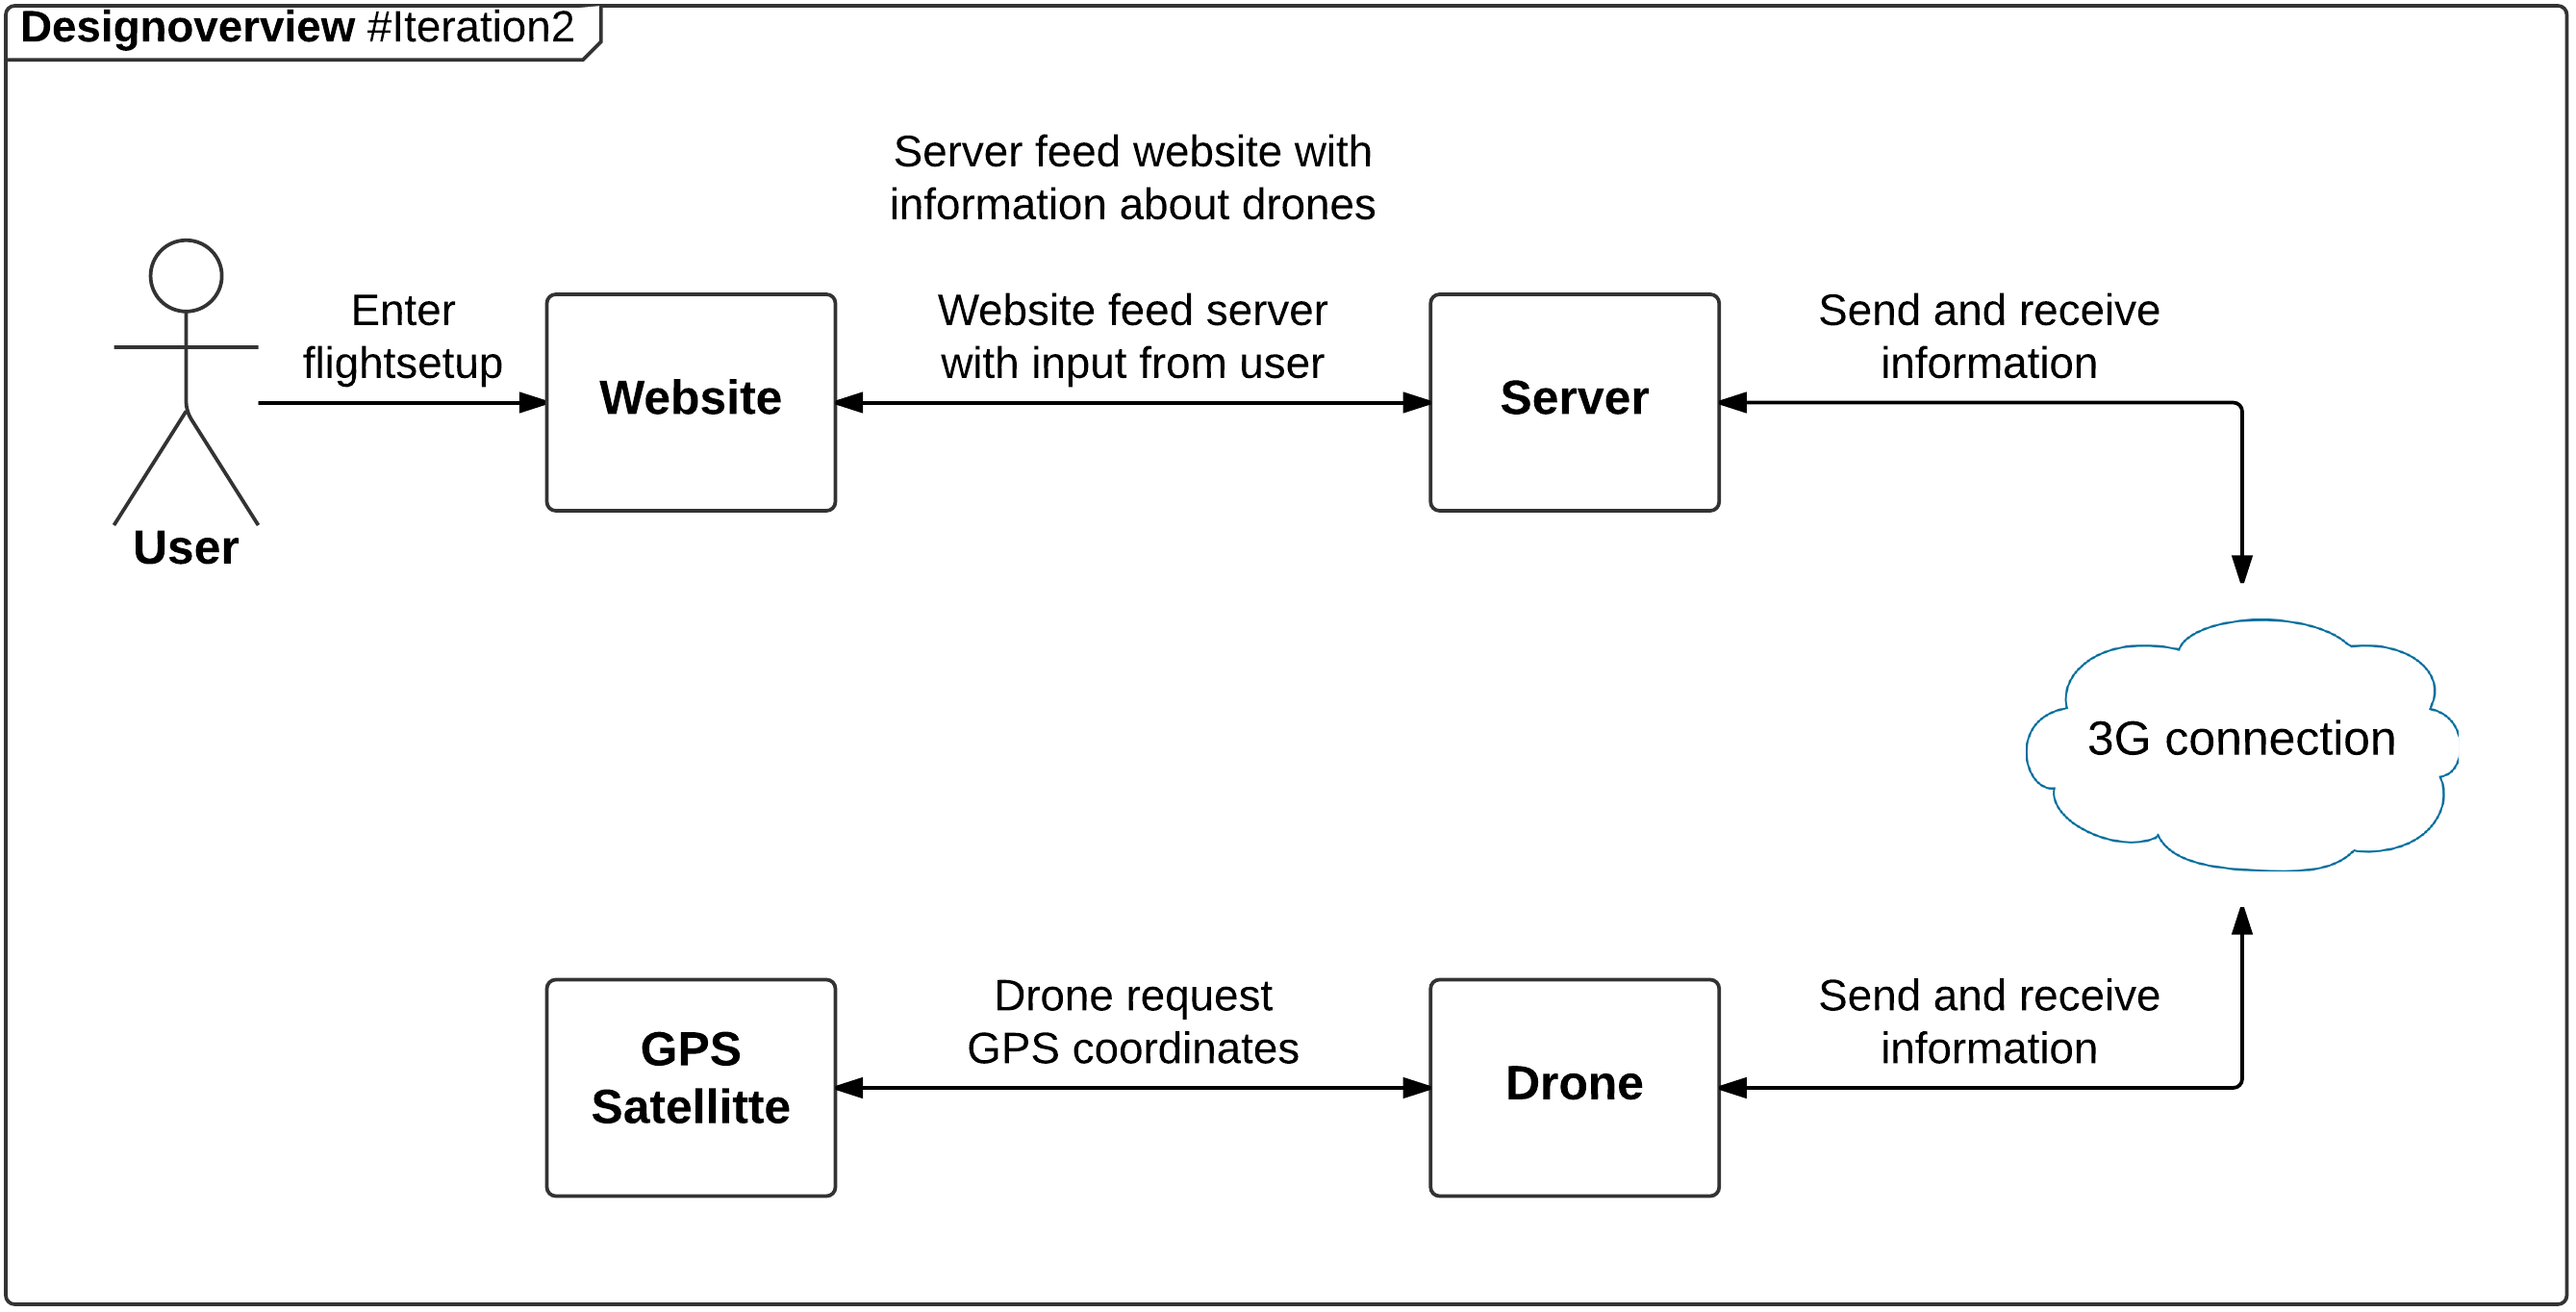
\includegraphics[width=1\textwidth]{Billeder/design_overview/design_overview_iteration2.png}
	\vspace{-.5cm}
	\caption{Designoverview \#iteration 2}
	\label{fig:design_overview_UC1}
\end{figure}


\newpage
\subsubsection*{Pakkediagram drone}
I dette afsnit vises pakkediagram tilhørende drone. De pakker der vises i pakkediagrammet består af en eller flere klasser, der med stort samspil udfører opgaver indenfor et fælles ansvarsområde. På hver pakke findes en lille beskrivelse, der tydeliggør pakkens ansvarsområde. De dele af pakkerne der er gråskraveret, er funktionalitet udarbejdet i tidligere iteration.


\begin{figure}[H]
	\centering
	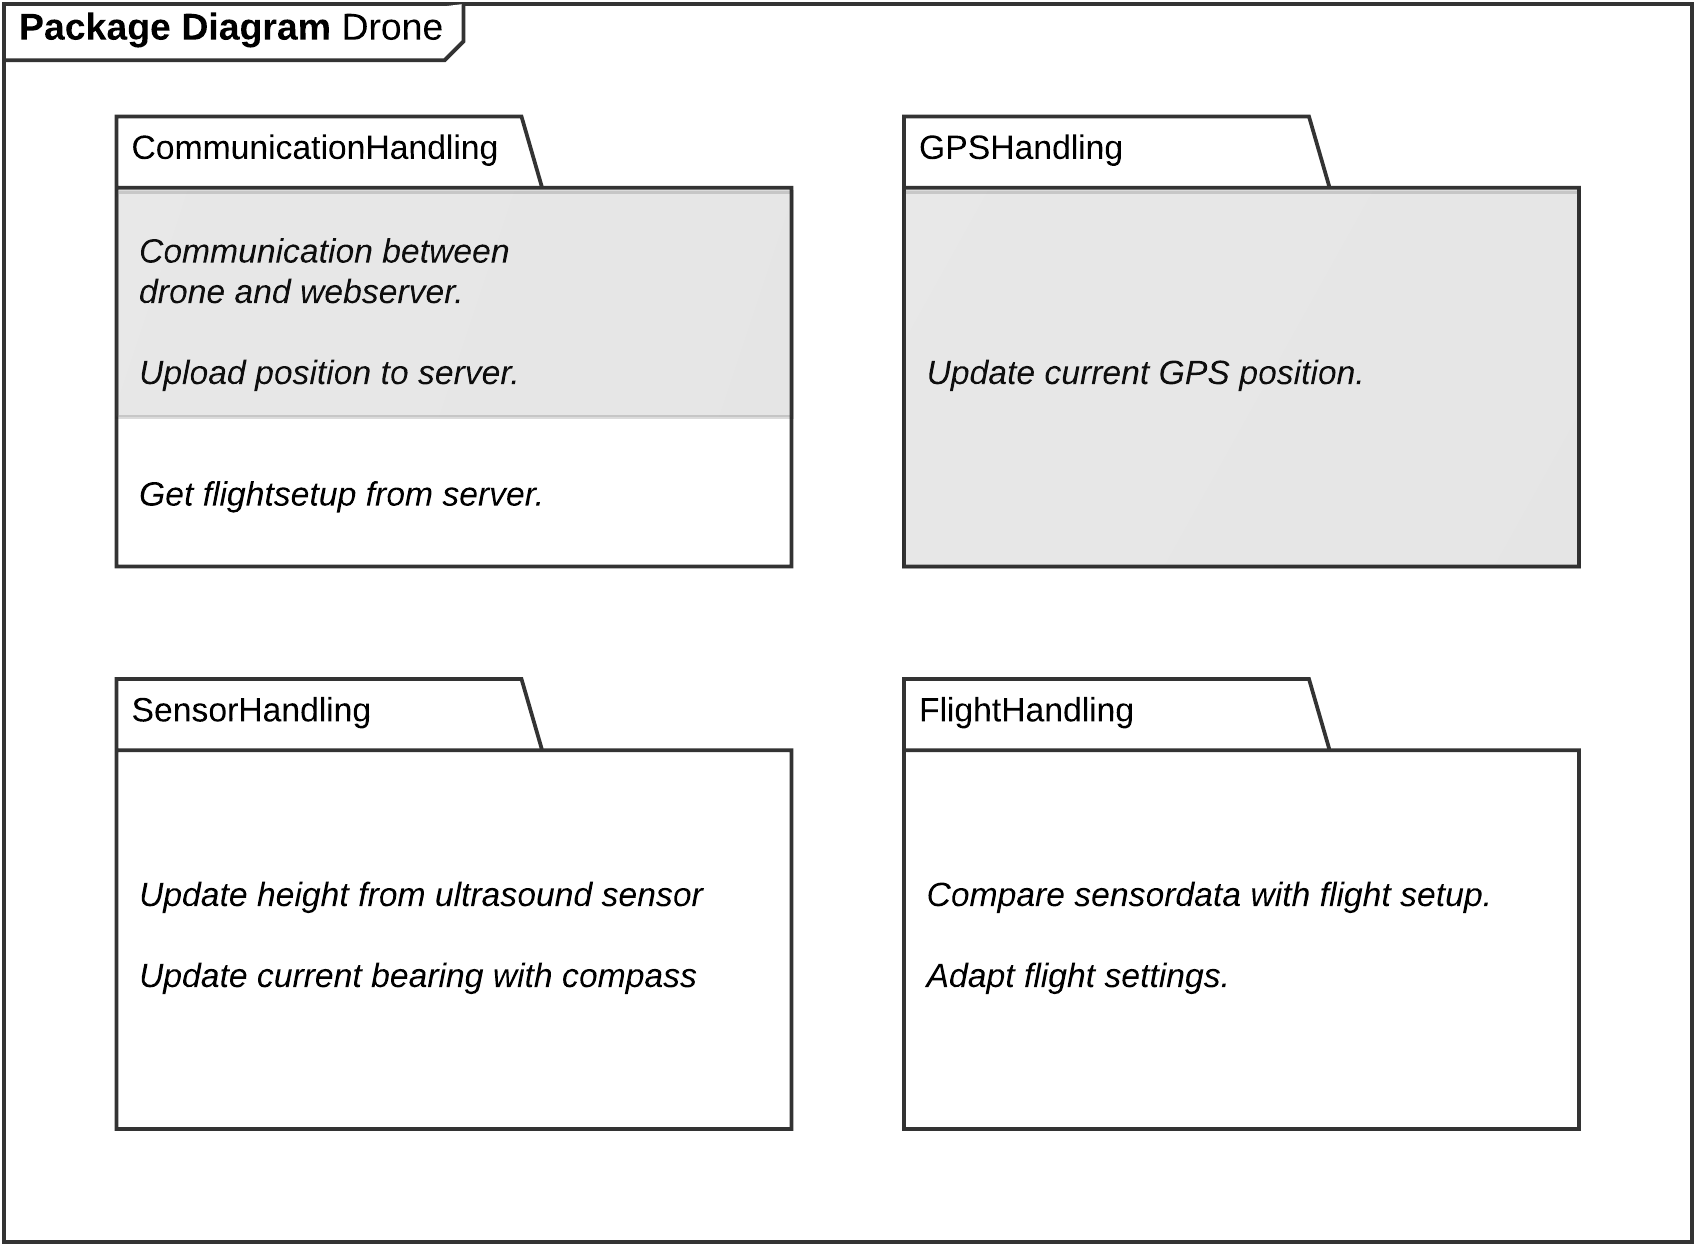
\includegraphics[width=1\textwidth]{Billeder/pakke_diagrammer/iteration2_drone.png}
	\vspace{-0.5cm}
	\caption{Pakkediagram drone}
	\label{fig:iteration2_pakke_diagram_drone}
\end{figure}

\textbf{CommunicationHandling}\\
Pakkens ansvar er kommunikation imellem drone og server. Efter denne iteration skal dronen både kunne hente flyveopsætninger fra server og sende sin nuværende GPS position til server.

\textbf{GPSHandling}\\
Pakkens ansvar er håndtering af GPS. Dels er pakken ansvarlig for opstart og initiering af GPS, og desuden bruges pakken hver gang dronens nuværende GPS position skal opdateres.

\textbf{SensorHandling}\\
Pakken er ansvarlig for indsamling af sensor data. I denne iteration skal pakken bruges til aflæsning af højdemåler og kompasset på flight control boardet. 

\textbf{FlightHandling}\\
Pakkens ansvar er kontrol og styring af drone under flyvning. Ved sammenligning af sensor data og data fra flyveopsætning tilpasses flyvehøjde, orientering mm



\newpage
\subsubsection*{Pakkediagram webapplikation}

I dette afsnit vises pakkediagram tilhørende webapplikation. De pakker der vises i pakkediagrammet består af en eller flere klasser, der med stort samspil udfører opgaver indenfor et fælles ansvarsområde. På hver pakke findes en lille beskrivelse, der tydeliggør pakkens ansvarsområde. De dele af pakkerne der er gråskraveret, er funktionalitet udarbejdet i tidligere iteration.

\begin{figure}[H]
	\centering
	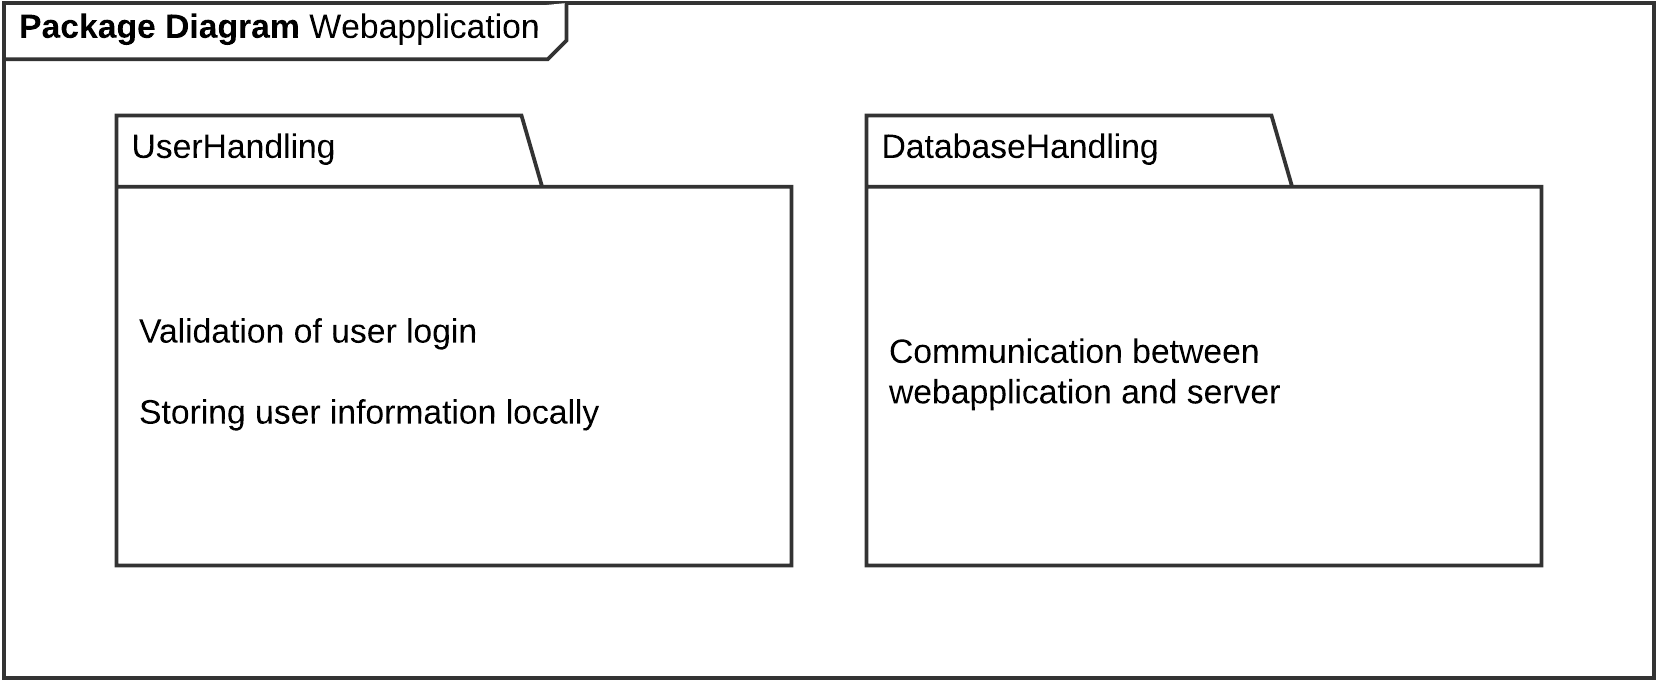
\includegraphics[width=1\textwidth]{Billeder/pakke_diagrammer/iteration1_server.png}
	\vspace{-0.5cm}
	\caption{Overordnet pakke diagram over webapplikationen}
	\label{fig:iteration1_pakke_diagram_webapp}
\end{figure}

\textbf{UserHandling}\\
Pakkens ansvar er validering af login/log ud på websitet. Pakken har også ansvaret for at hente og gemme data om den pågældende bruger.

\textbf{DatabaseHandling}\\
Pakkens ansvar er kommunikation imellem databasen og serveren. 

\textbf{DroneHandling}\\
Pakkens ansvar er alt data vedrørende dronen, så som håndteringen af events, waypoints og div droner.

\newpage

\subsubsection*{Sekvensdiagram drone}

Til iteration 2 er systemsekvensen beskrevet med 3 mindre sekvensdiagrammer i stedet for 1 stort. Ydermere er der lavet 2 sekvens diagrammer der går mere i dybden med 3G modulet og dens klasser. 
Denne fremstilling gør det muligt at repræsentere systemets funktionalitet på mere overskuelig vis, hvilket indirekte øger forståelsen af diagrammerne. Hvert af de 3 overordnede sekvensdiagrammer bruges til at fortælle hvordan en delmængde af systemet fungerer.

Af figur \ref{fig:Sekvens_diagram_iteration2_1} fremgår det hvordan bruger opretter en ny flyveopsætning. Det vises desuden hvilke interaktioner der foretages mellem bruger og website, samt hvordan server løbende indgår og benyttes i sekvensen. 

%kommentar
\begin{figure}[H]
	\centering
	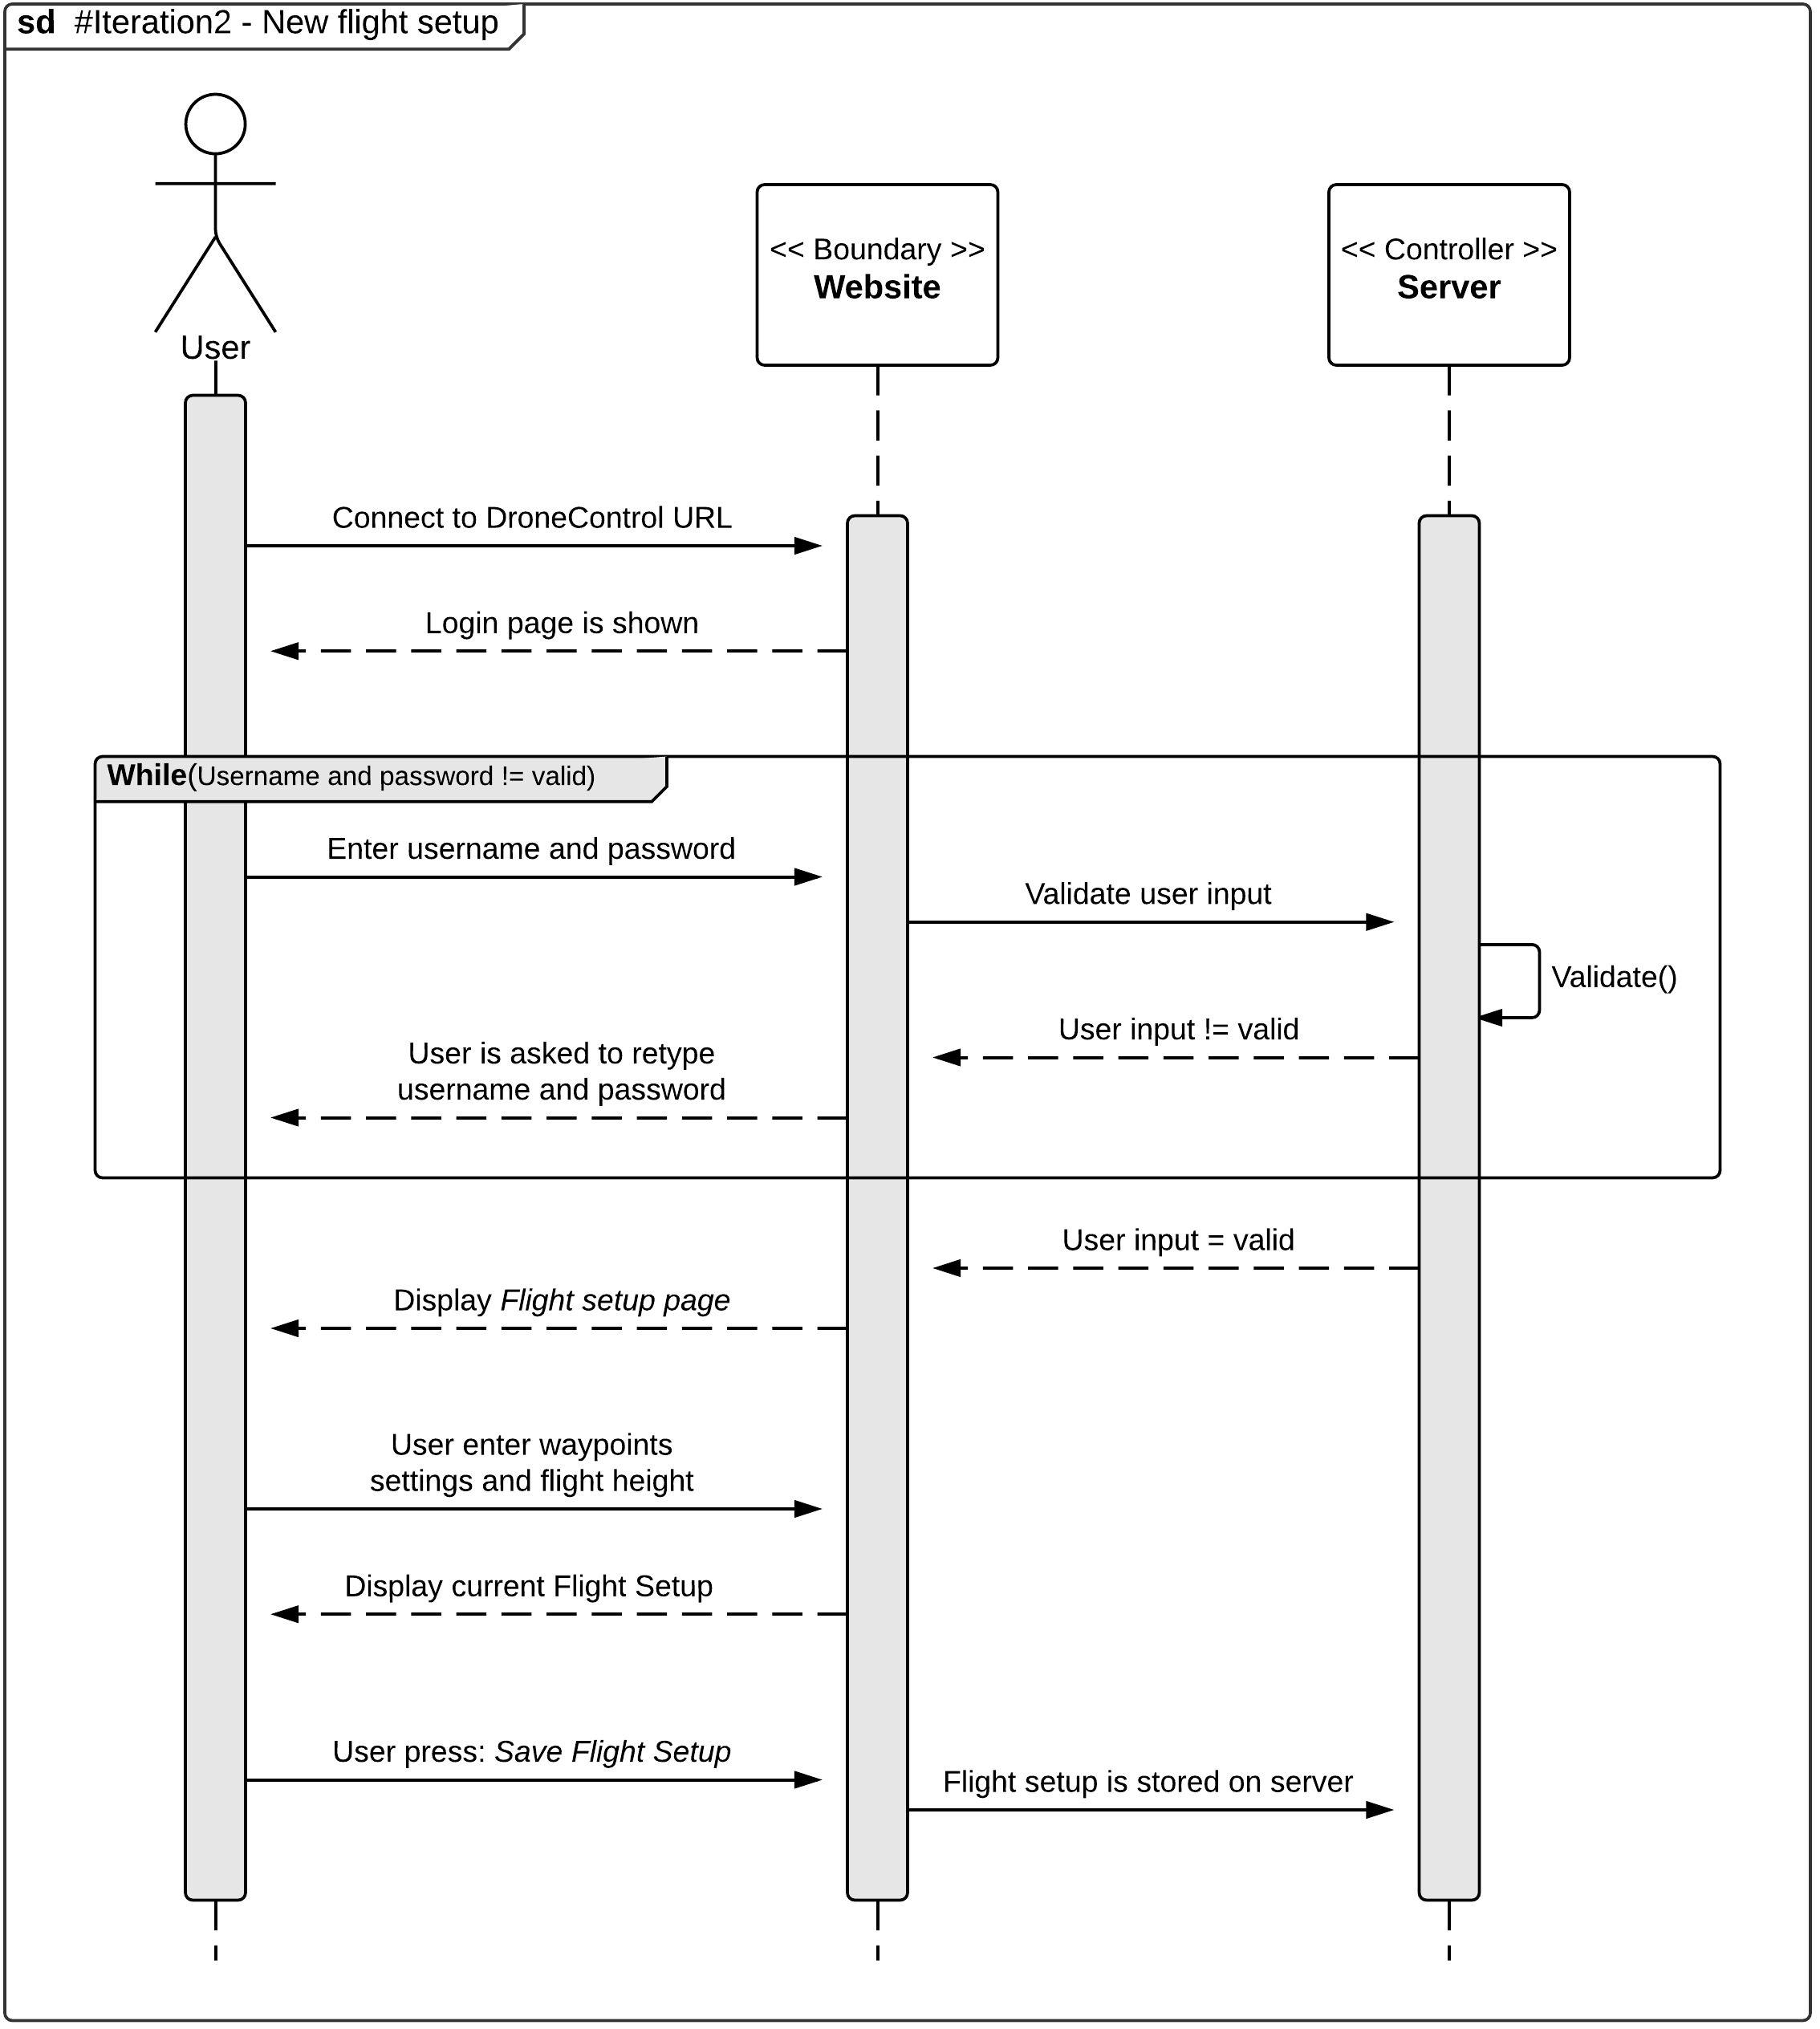
\includegraphics[width=1\textwidth]{Billeder/sekvens/sekvens_iteration2_1}
	\caption{Sekvensdiagram \#iteration 2}
	\label{fig:Sekvens_diagram_iteration2_1}
\end{figure}


\newpage

På figur \ref{fig:Sekvens_diagram_iteration2_2} fremgår det hvordan dronens main controller via 3G-shieldet kommunikerer med serveren for at kontrollere om der er en ny flyveopsætning tilgængelig. Det vises også hvilke beskeder der flyder frem og tilbage mellem main controller og server. Desuden vises det at dronen først henter ny flyveomsætning, når serveren har bekræftet, at der er en flyveopsætning tilgængelig.   

%kommentar
\begin{figure}[H]
	\centering
	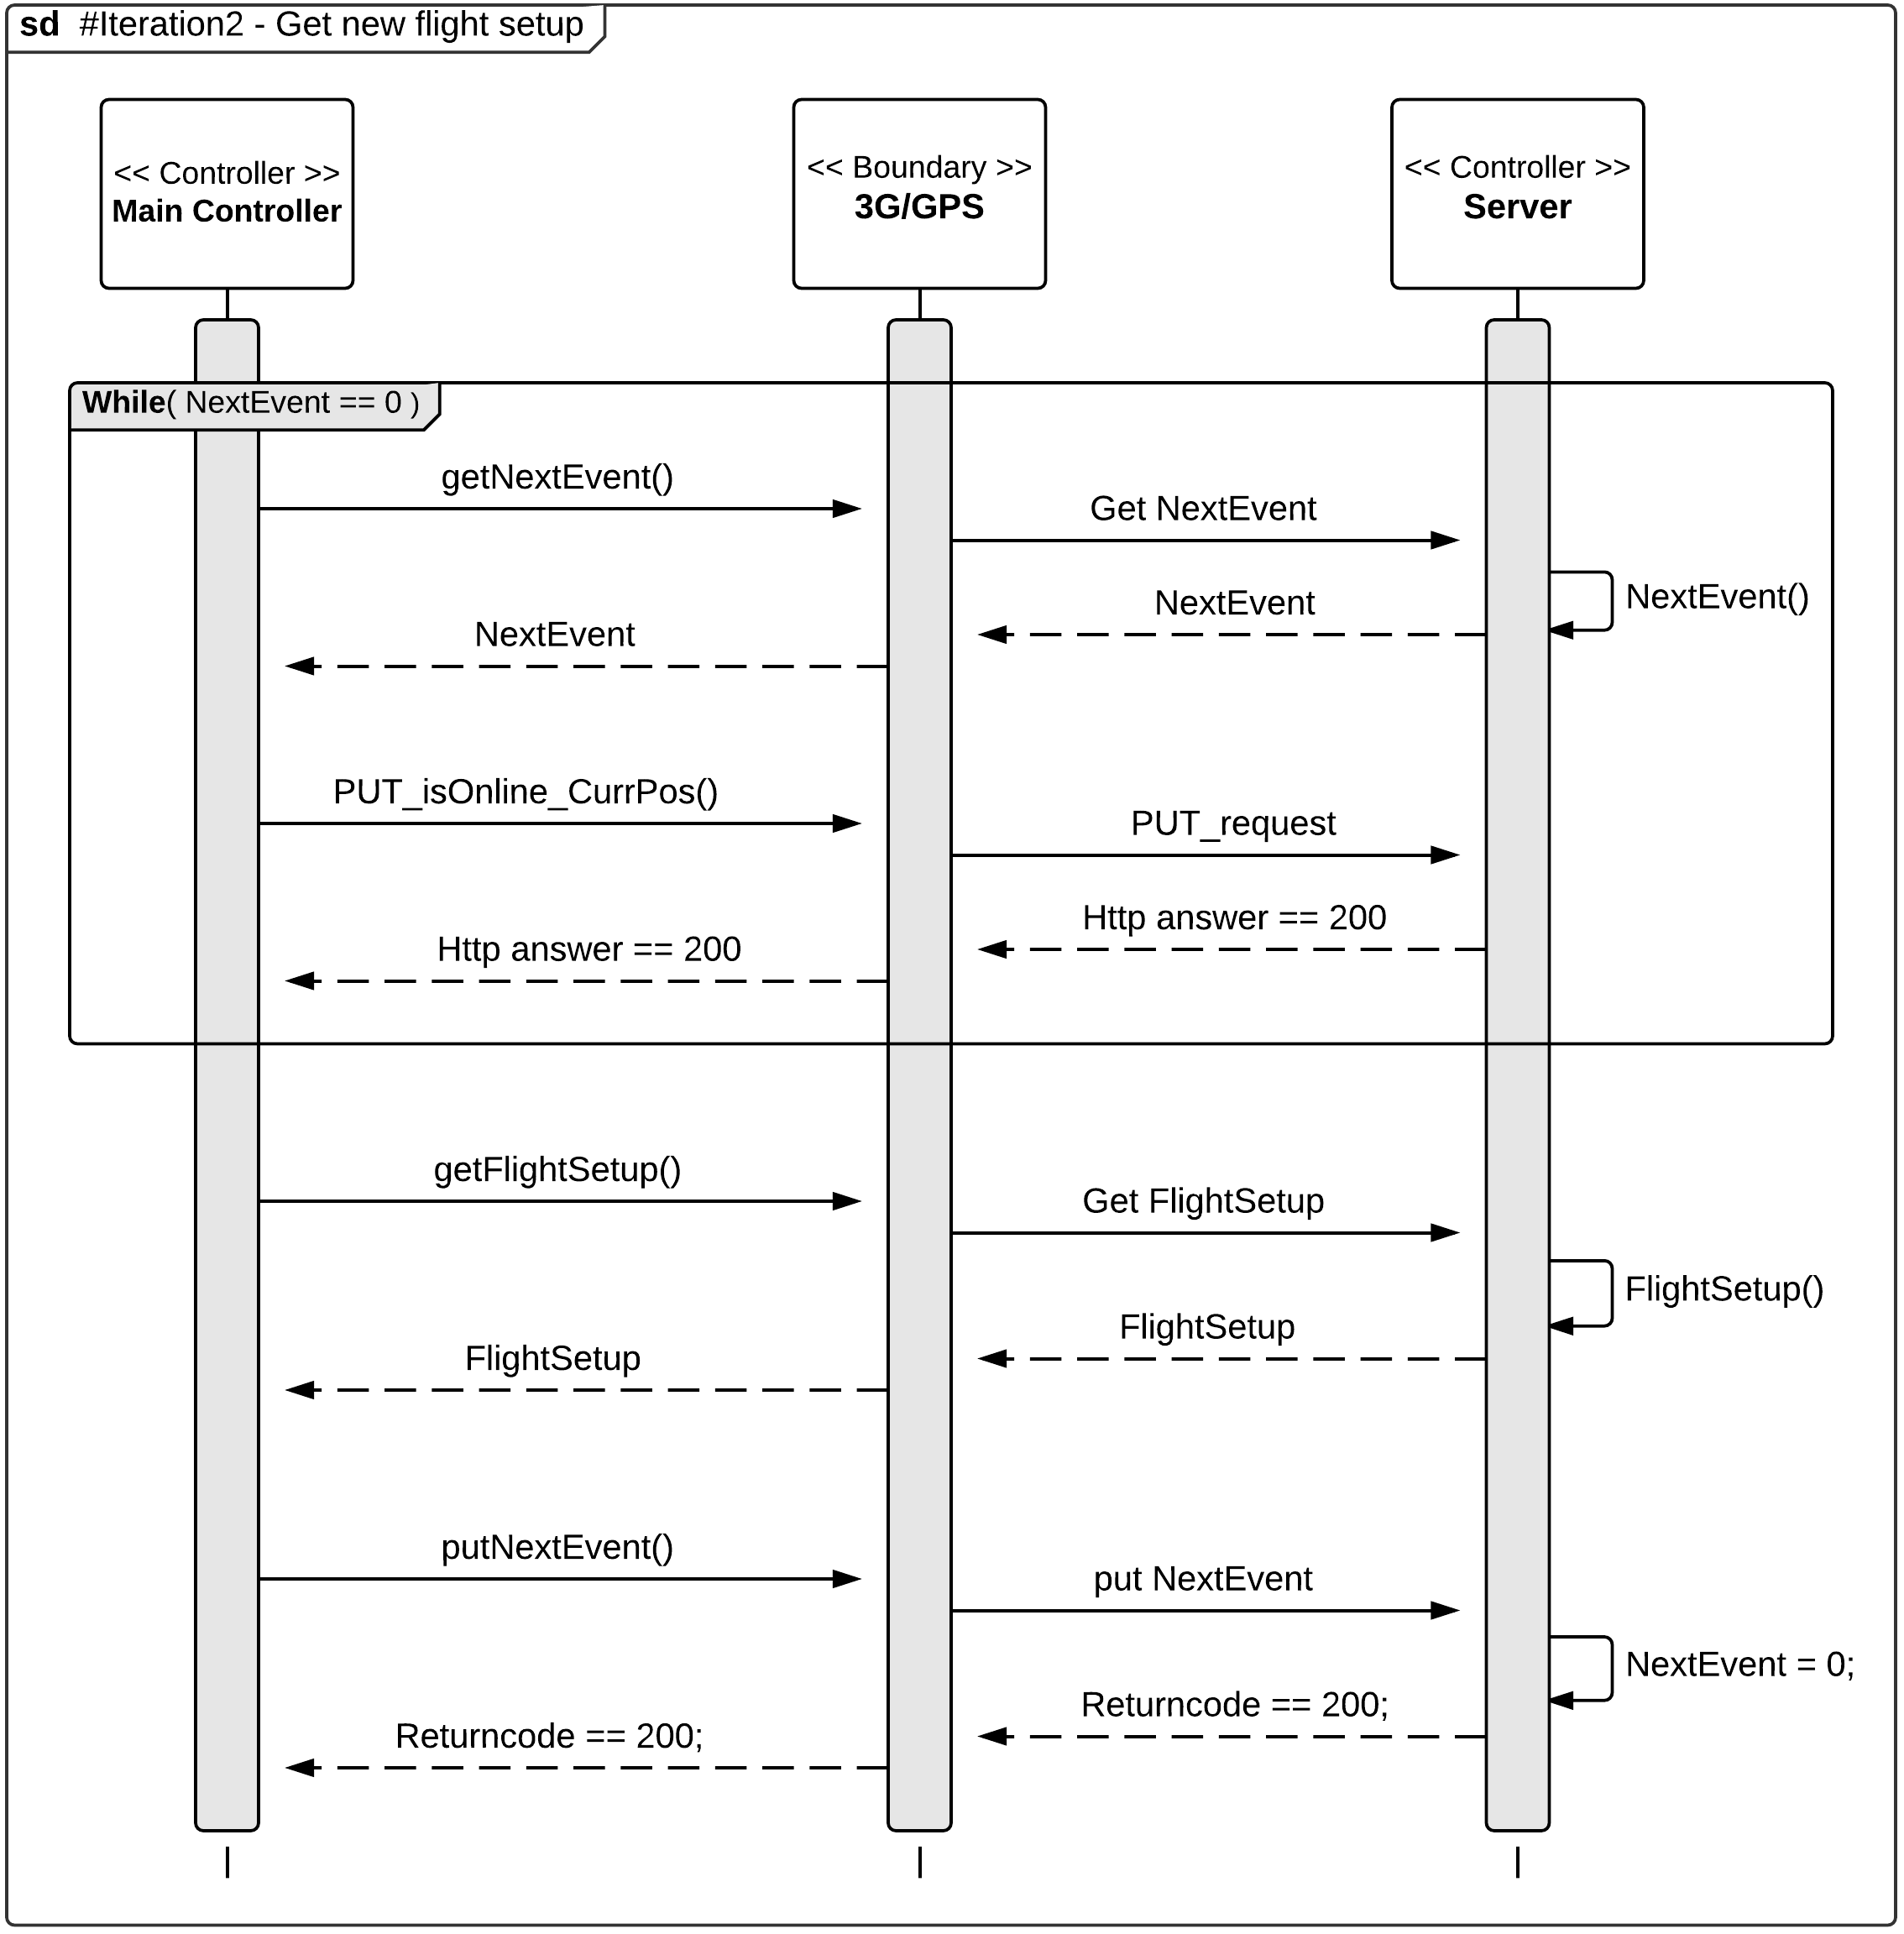
\includegraphics[width=1\textwidth]{Billeder/sekvens/sekvens_iteration2_2}
	\caption{Sekvensdiagram \#iteration 2}
	\label{fig:Sekvens_diagram_iteration2_2}
\end{figure}

\newpage

På Figur \ref{fig:Sekvens_getwaypoints} ses en mere detaljeret beskrivelse af 3G modulets klasser. Disse klasser håndterer al kommunikation mellem drone og server.

\begin{figure}[H]
	\centering
	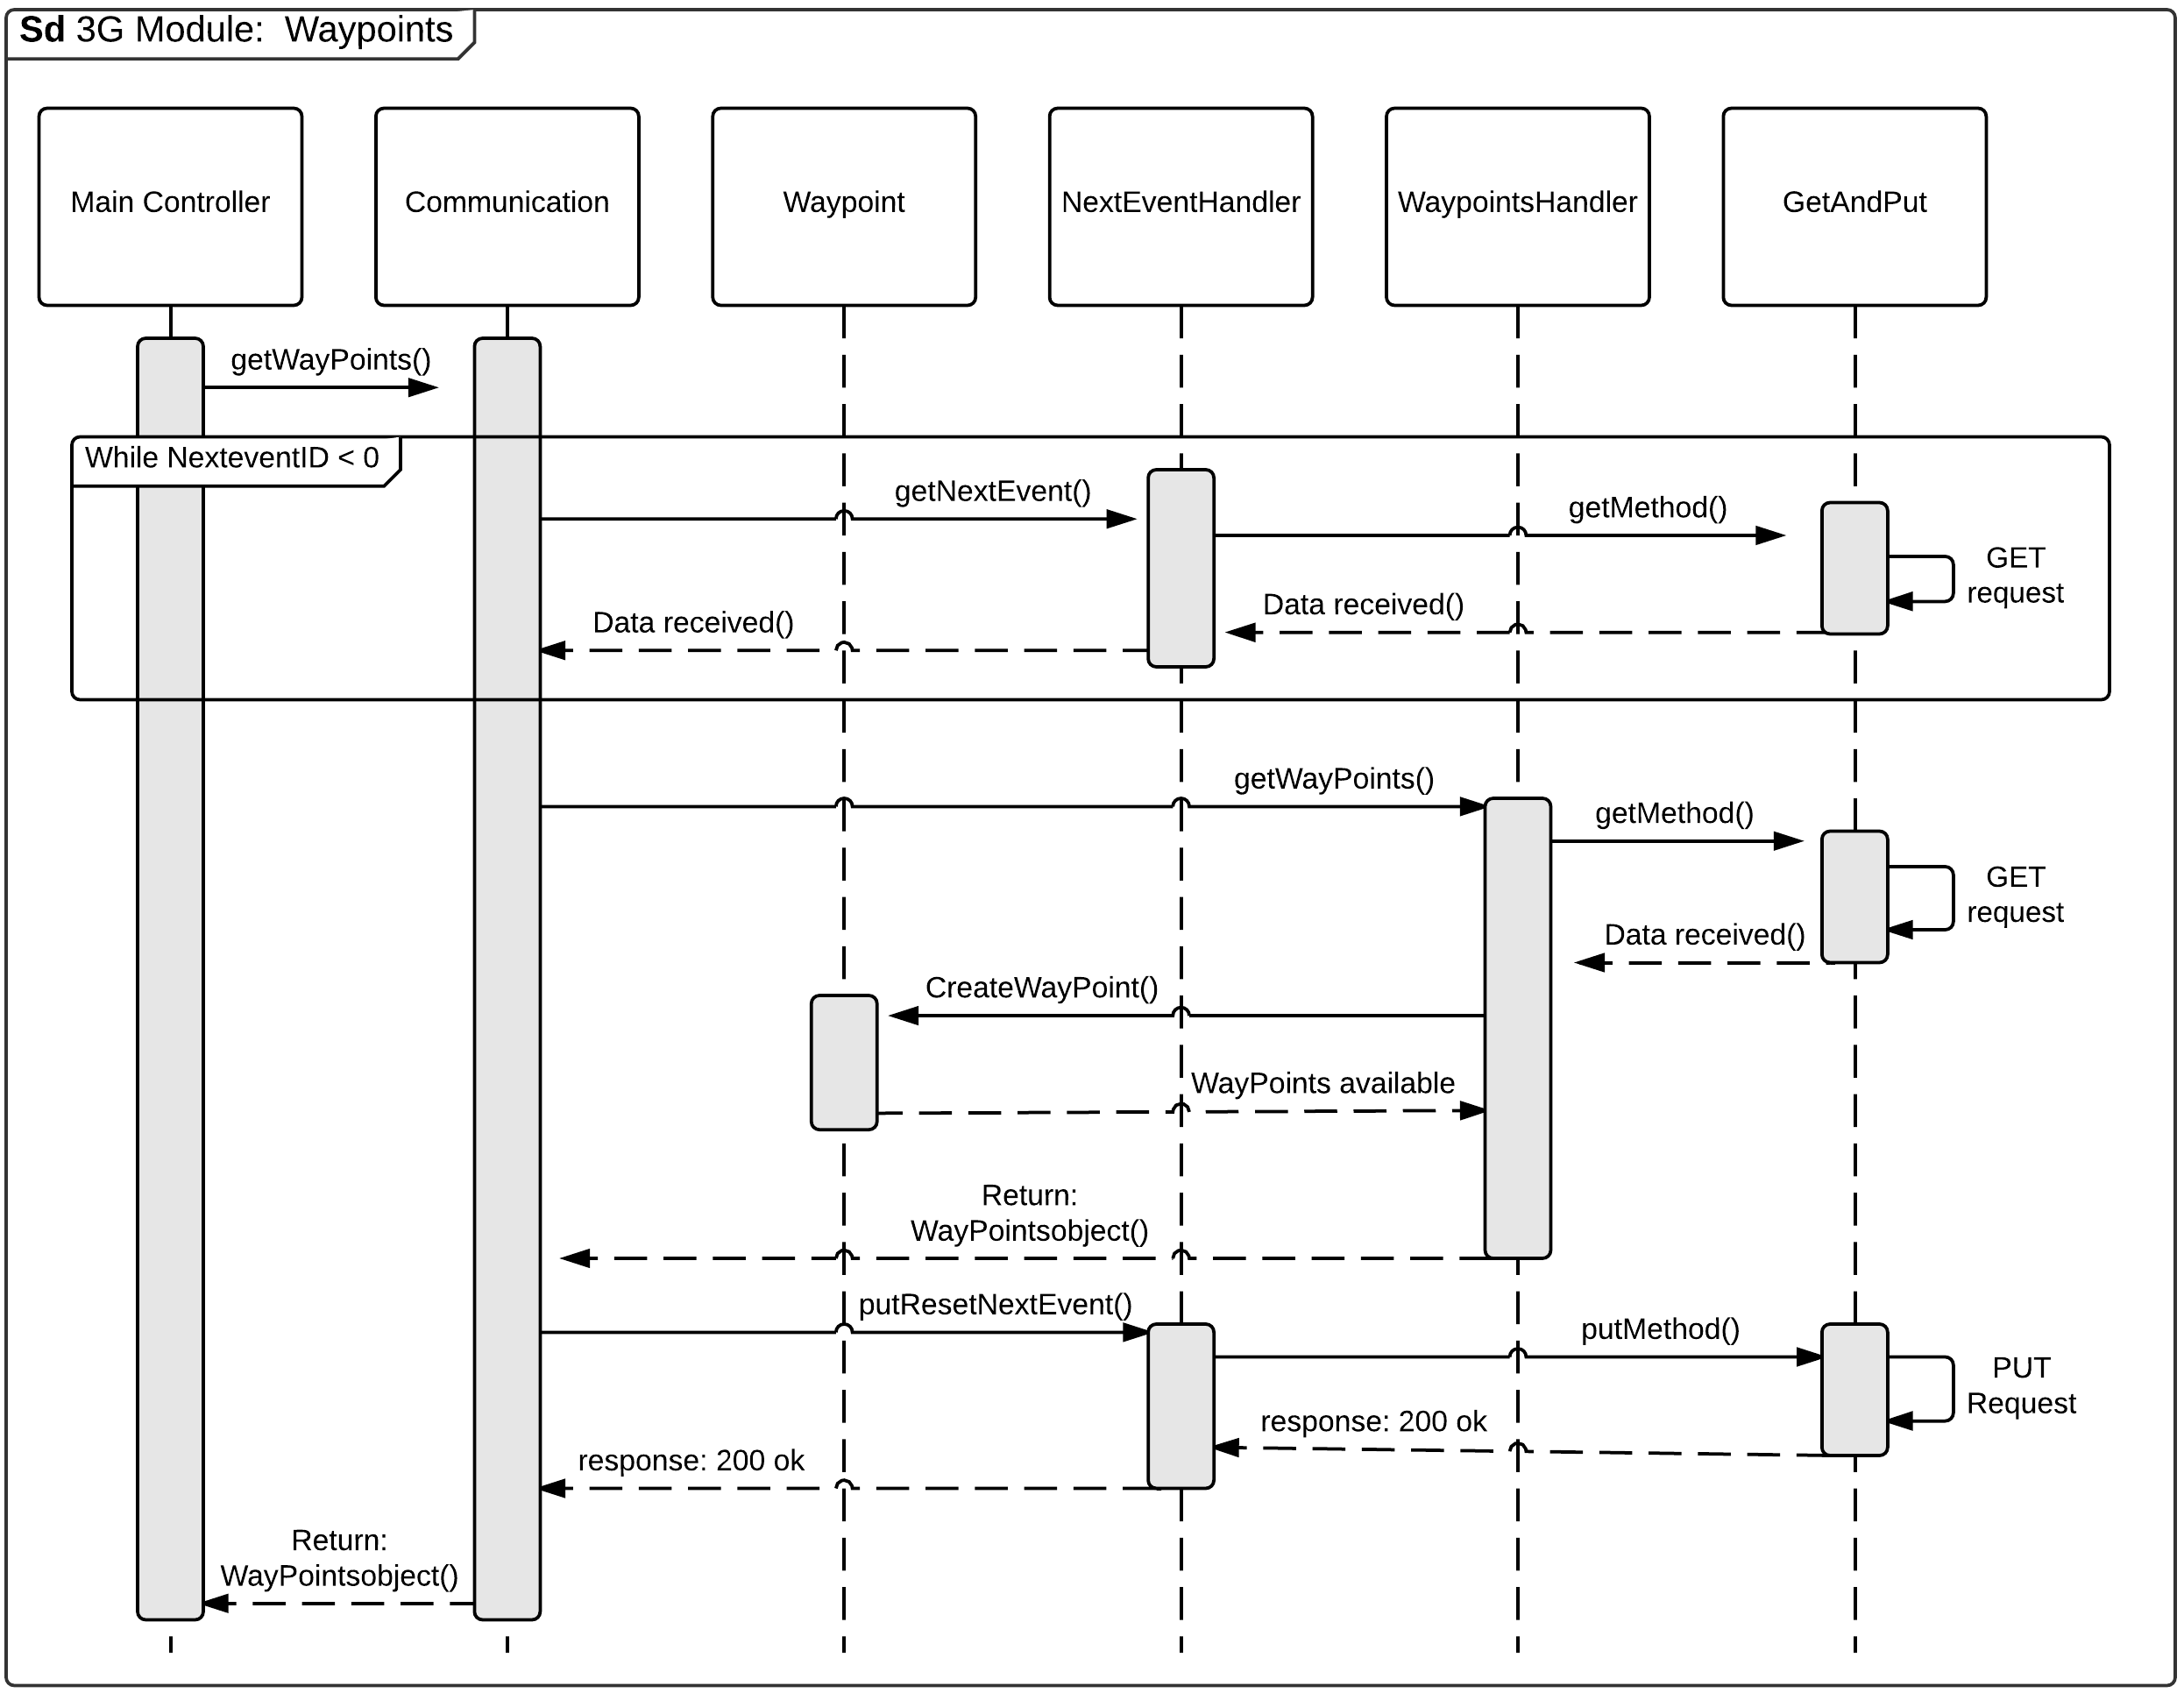
\includegraphics[width=1\textwidth]{Billeder/sekvens/sekvens_getwaypoints.png}
	\caption{Sekvensdiagram udvidet 3G module - getwaypoints}
	\label{fig:Sekvens_getwaypoints}
\end{figure}

\newpage

Af figur \ref{fig:Sekvens_diagram_iteration2_3} fremgår det hvordan dronen opererer når den flyver autonomt mod en givet GPS position. Main controlleren indsamler kompas data fra flight control boardet, latitude og longitude fra 3G/GPS modulet og flyvehøjde fra ultralyds sensoren. Den indhentede data processeres og bruges til at korrigerer de nuværende flyveindstillinger.
Som det fremgår af while loopet fortsætter flyvningen indtil dronen er 15 meter fra den GPS destination bruger valgte i flyveopsætningen. 


%kommentar
\begin{figure}[H]
	\centering
	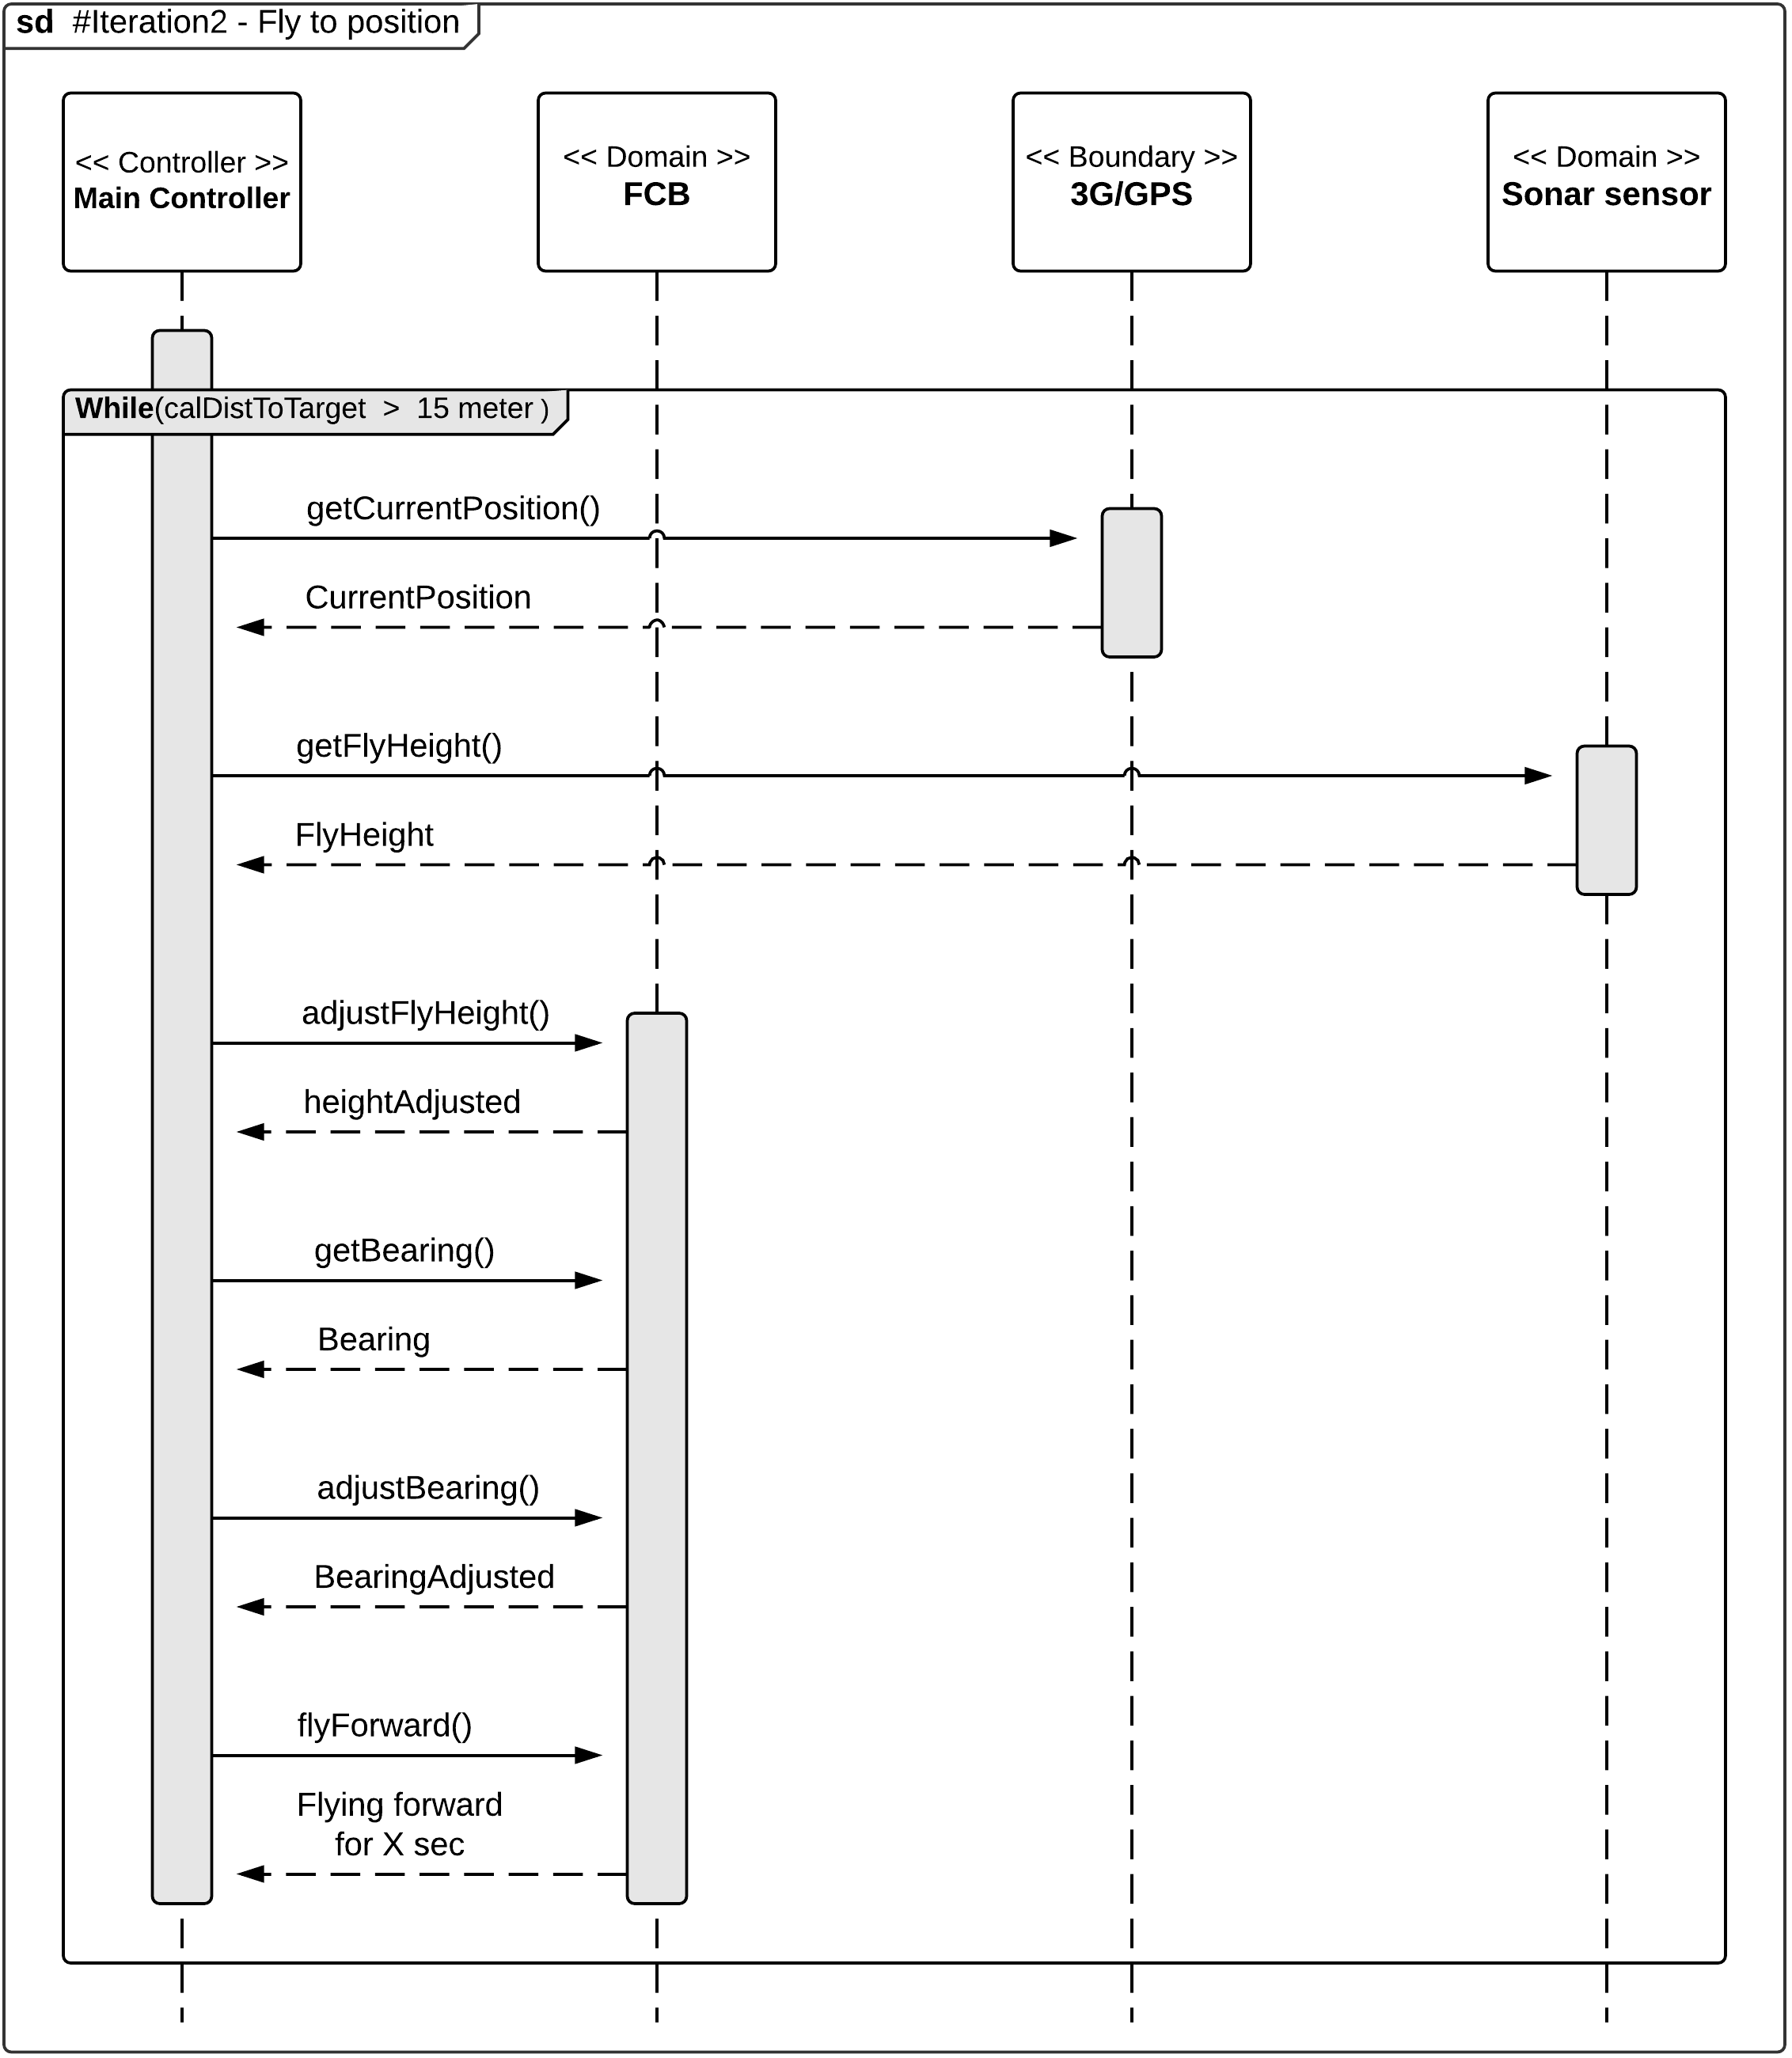
\includegraphics[width=1\textwidth]{Billeder/sekvens/sekvens_iteration2_3}
	\caption{Sekvensdiagram \#iteration 2}
	\label{fig:Sekvens_diagram_iteration2_3}
\end{figure}

\newpage
\subsubsection*{Sekvensdiagram webapplikation}
\vspace{-0.1cm}
På figur \ref{fig:page_load} ses hvordan klasserne på websitet interagere med hinanden ved et page load. Kortet bliver initialiseret med centrum over århus og drone markeren bliver initialiseret. Useren som blev gemt ved login bliver brugt til at give en velkomst besked oppe i højre hjørne og sener vil blive brugt når der skal oprettet nye events. Listen med tilgængelige droner bliver loaded. Et click event bliver også oprettet som trigger ved click på kortet til oprettelse af nye waypoints.
\begin{figure}[H]
	\centering
	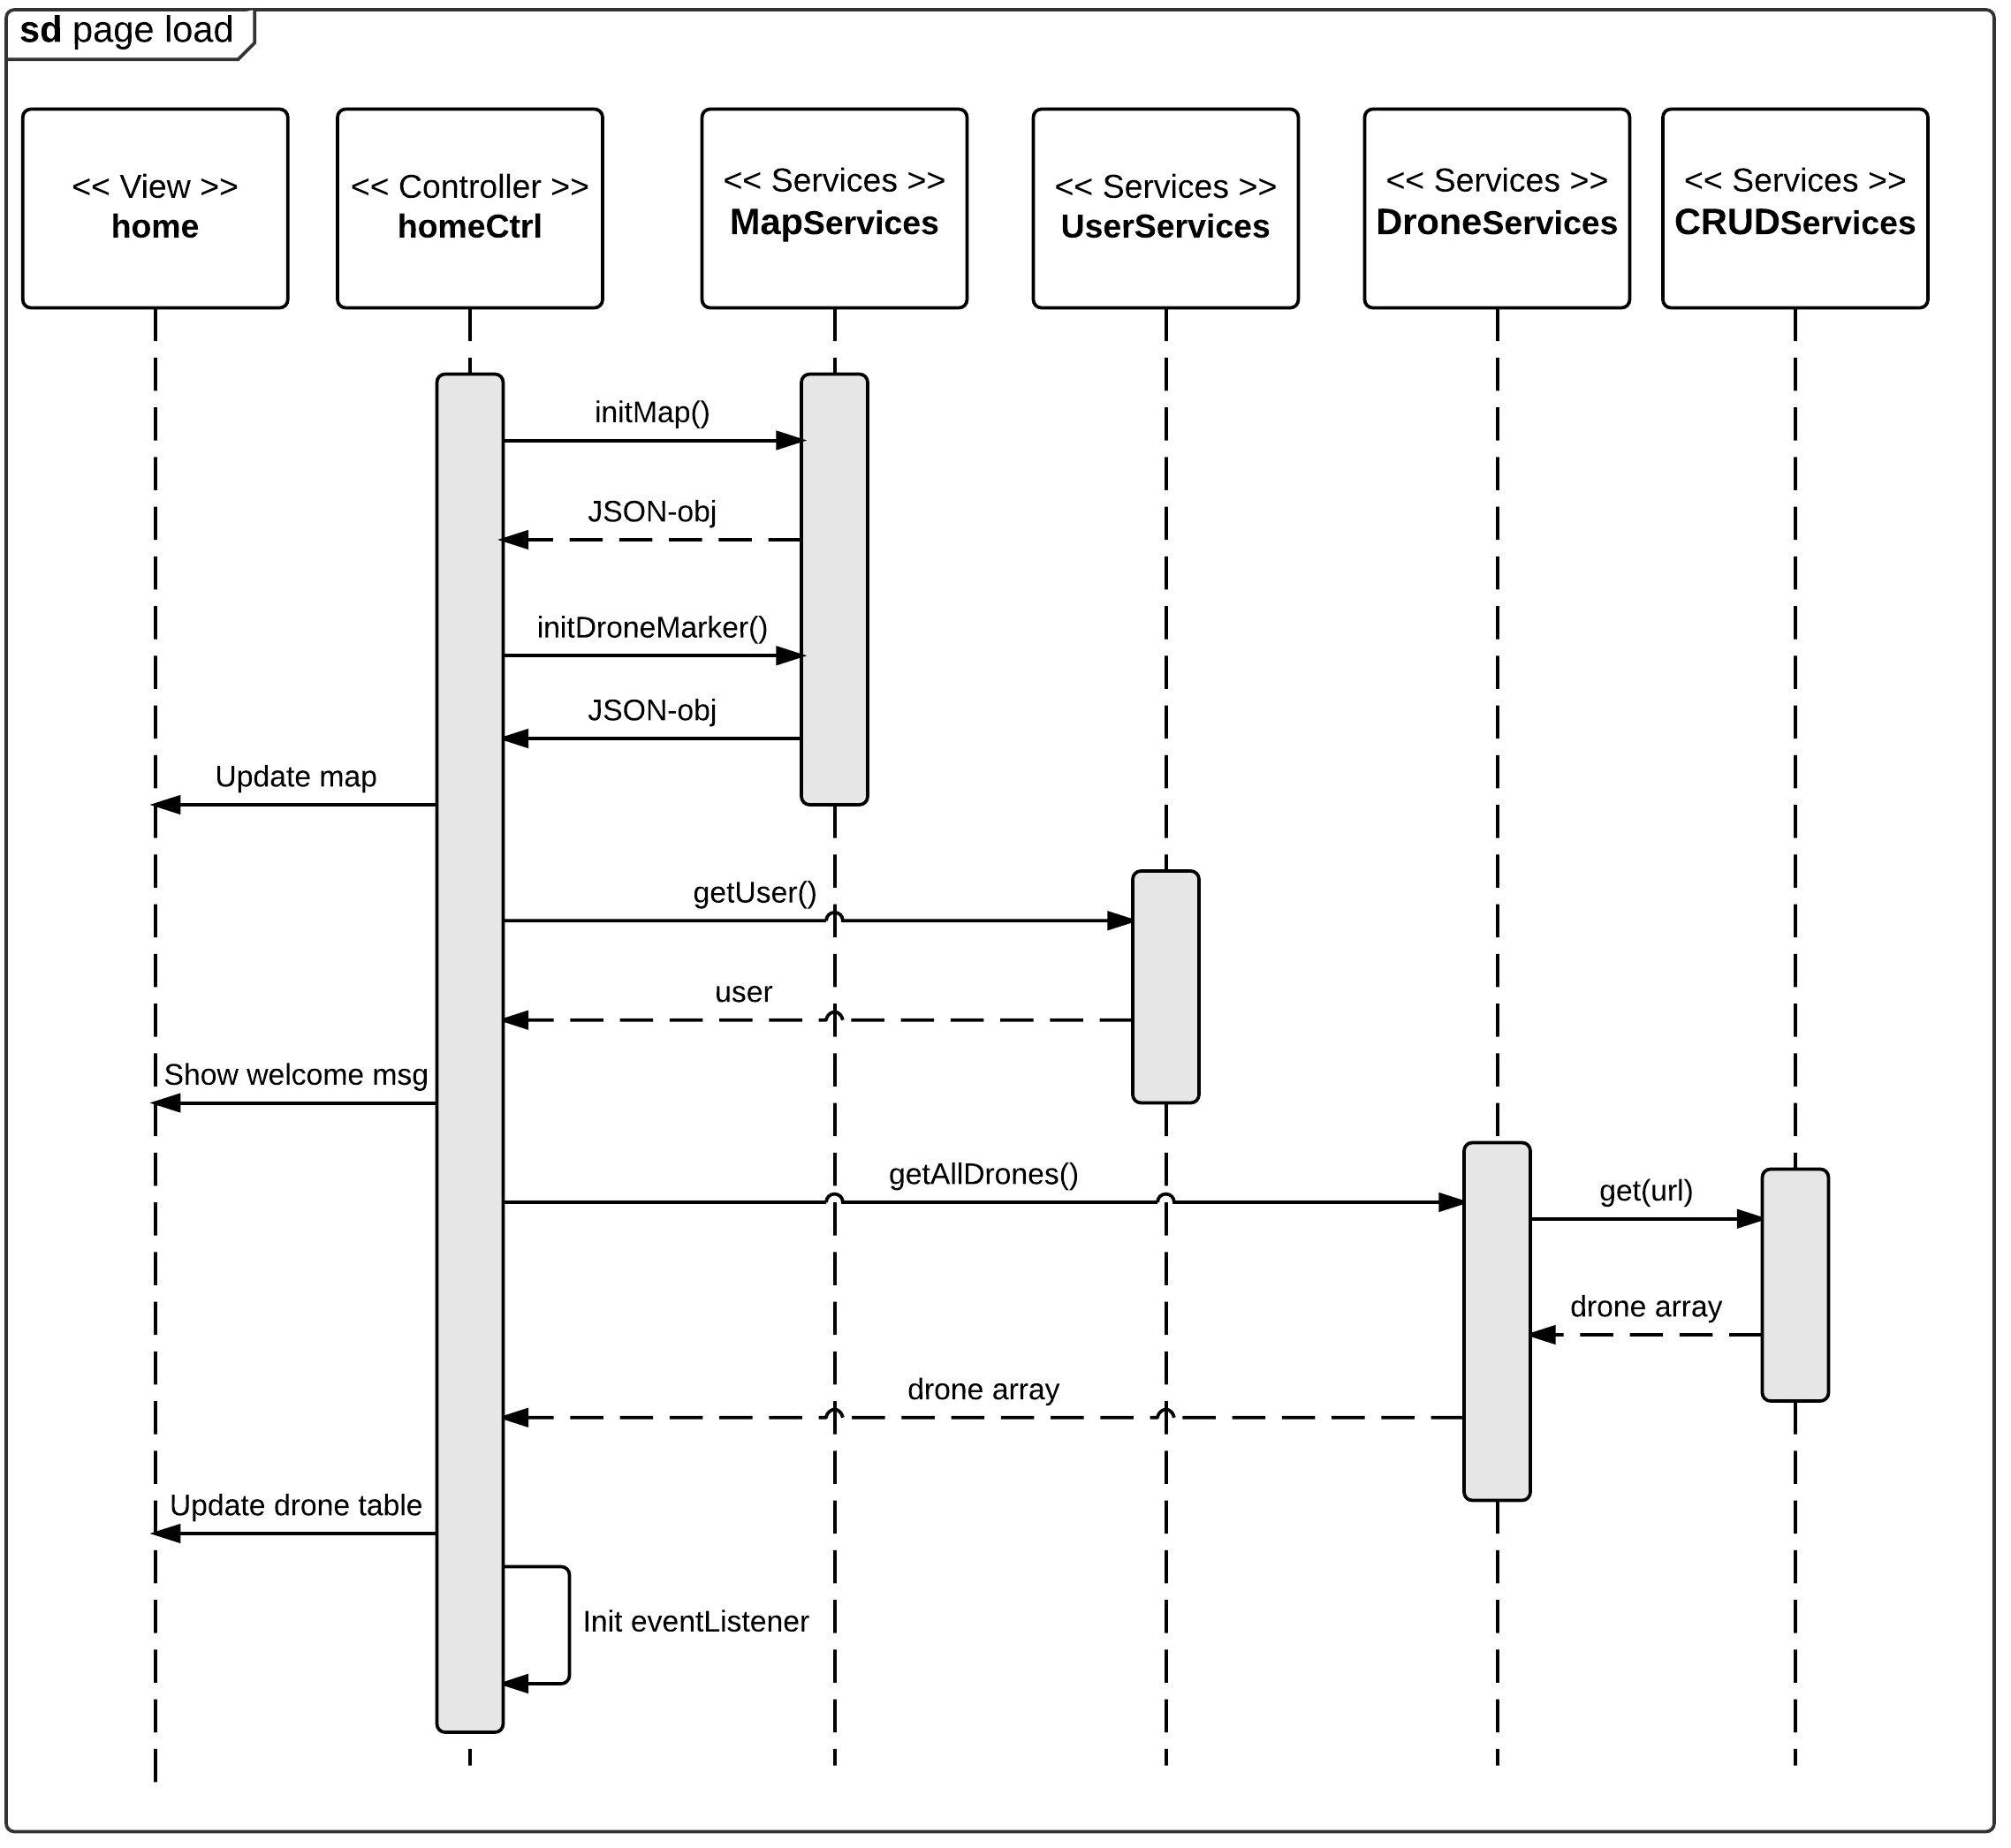
\includegraphics[width=1\textwidth]{Billeder/sekvens/sd_page_load.png}
	\caption{Sekvensdiagram page load}
	\label{fig:page_load}
\end{figure}

\newpage
På figur \ref{fig:send_waypoints} ses hvilke hændelser der finder sted i systemet, når useren trykker på "send event". Hvert services har et ansvar og det er dem der kommunikere ud til CRUD-servicesen, på den måde er logikken for data håndtering skubbet ud i div. services. 
\begin{figure}[H]
	\centering
	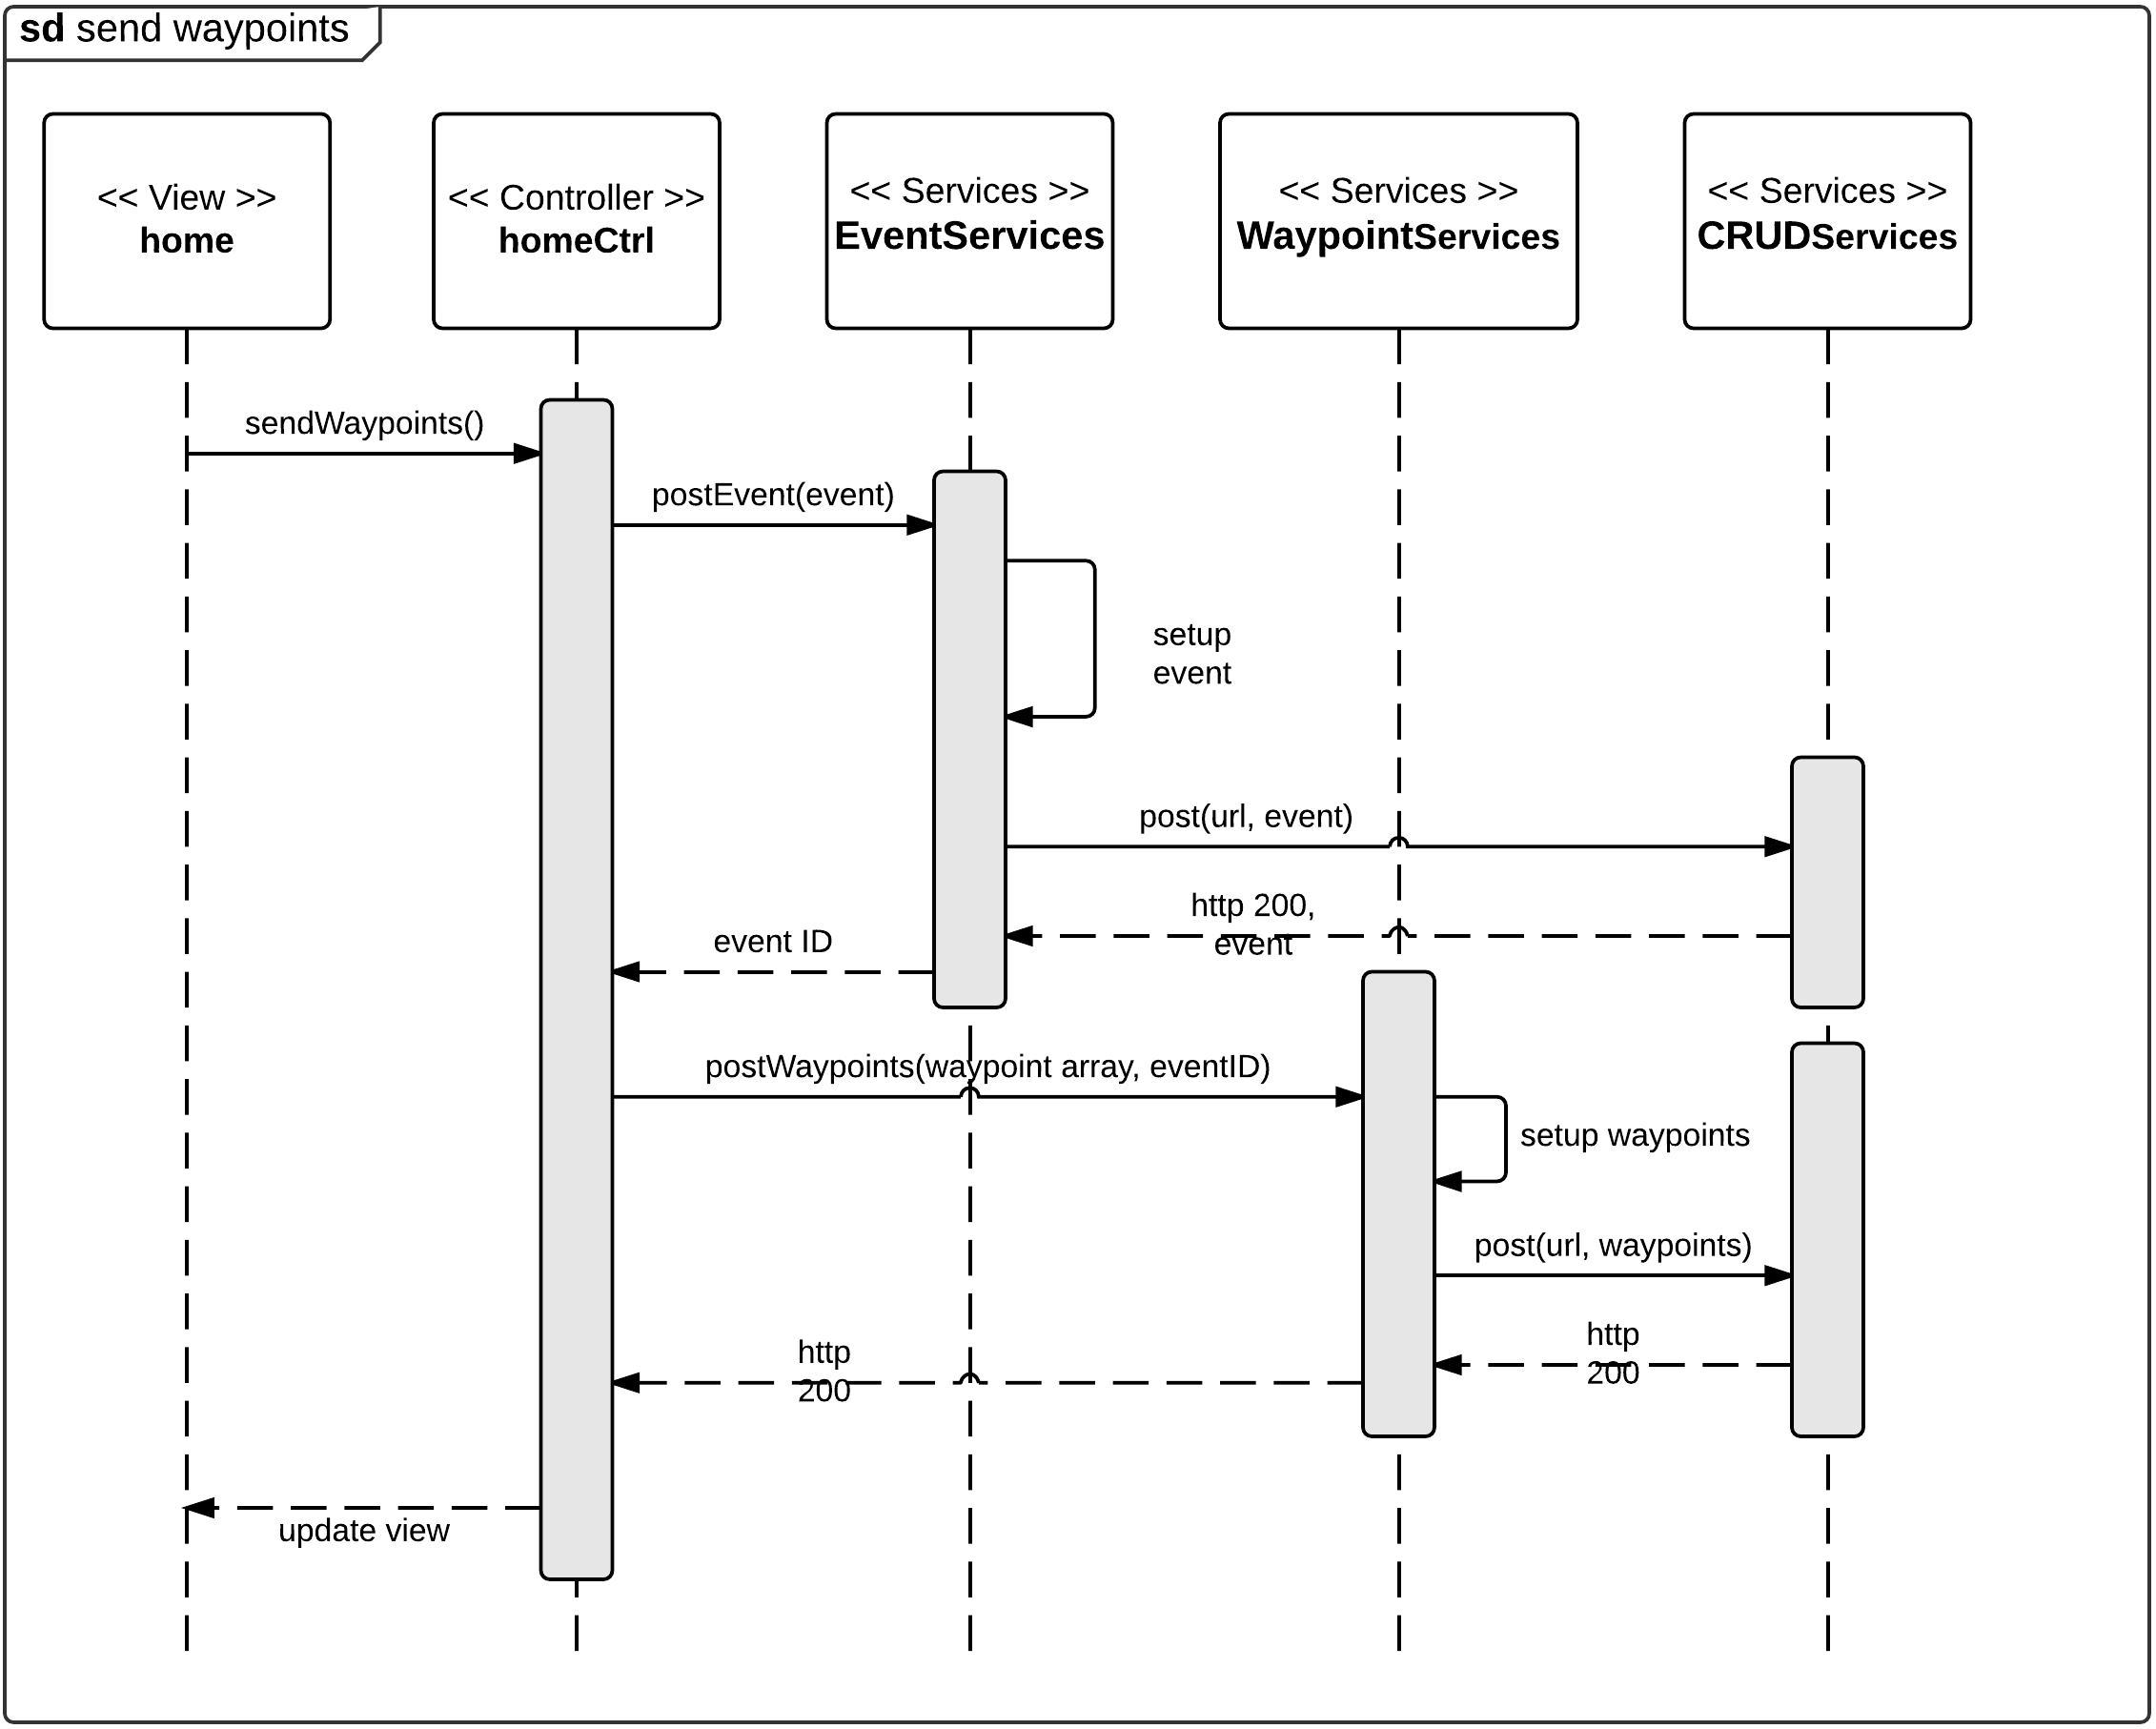
\includegraphics[width=1\textwidth]{Billeder/sekvens/sd_send_waypoints.png}
	\caption{Sekvensdiagram send waypoints}
	\label{fig:send_waypoints}
\end{figure}

\newpage
På figur \ref{fig:update_view} ses hvilke hændelser der finder sted i systemet, når useren trykker på forskellige droner i tabellen. Når et klik på tabellen finder sted skal view'et opdateret i forhold til den givet drone, dvs. hvis dronen har et event, så skal det vises og dertilhørende waypoints. Hvis der ikke er noget event tilknyttet til dronen skal useren have mulighed for at oprette et nyt event.
\begin{figure}[H]
	\centering
	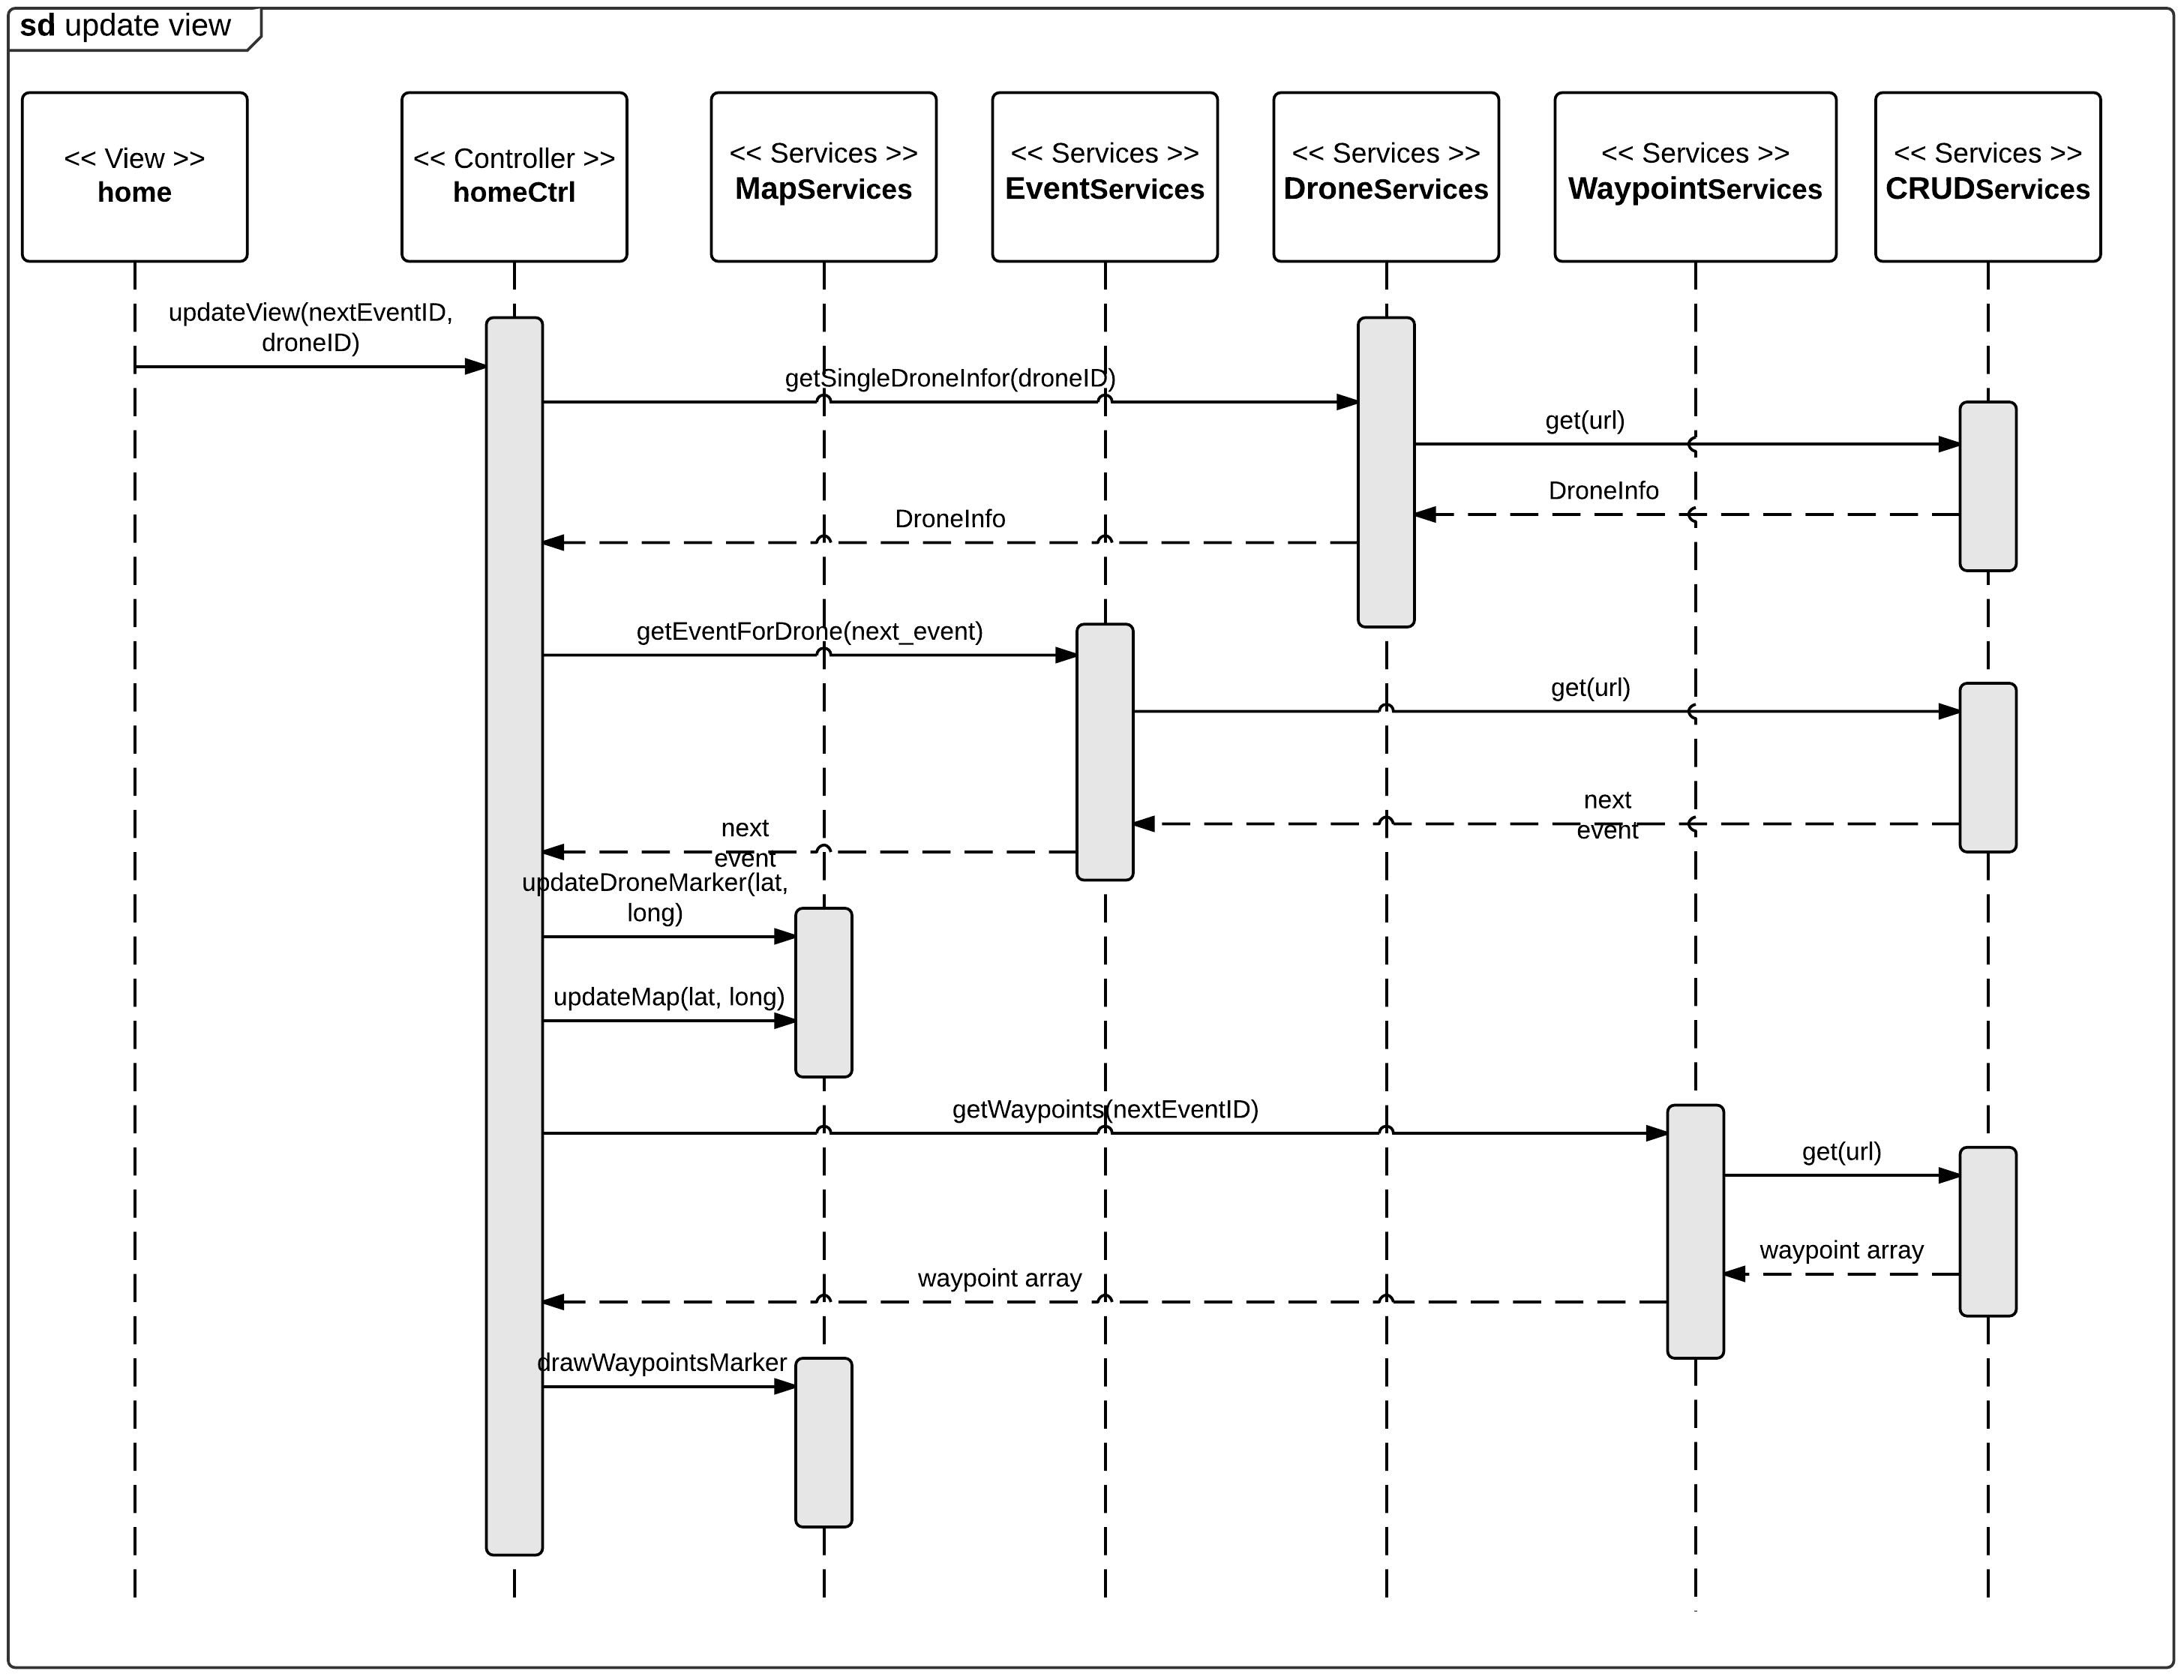
\includegraphics[width=1\textwidth]{Billeder/sekvens/sd_update_view.png}
	\caption{Sekvensdiagram opdater }
	\label{fig:update_view}
\end{figure}

\newpage
\subsubsection*{Klassediagram drone}

På figur \ref{fig:classDiagram_drone_underflyvning} ses klasse diagrammet for dronen. Det er klasserne der bruges af dronen, når den er flyve klar. På den følgende side er der en forklaring af klasserne og deres metoder. 

\begin{figure}[H]
	\centering
	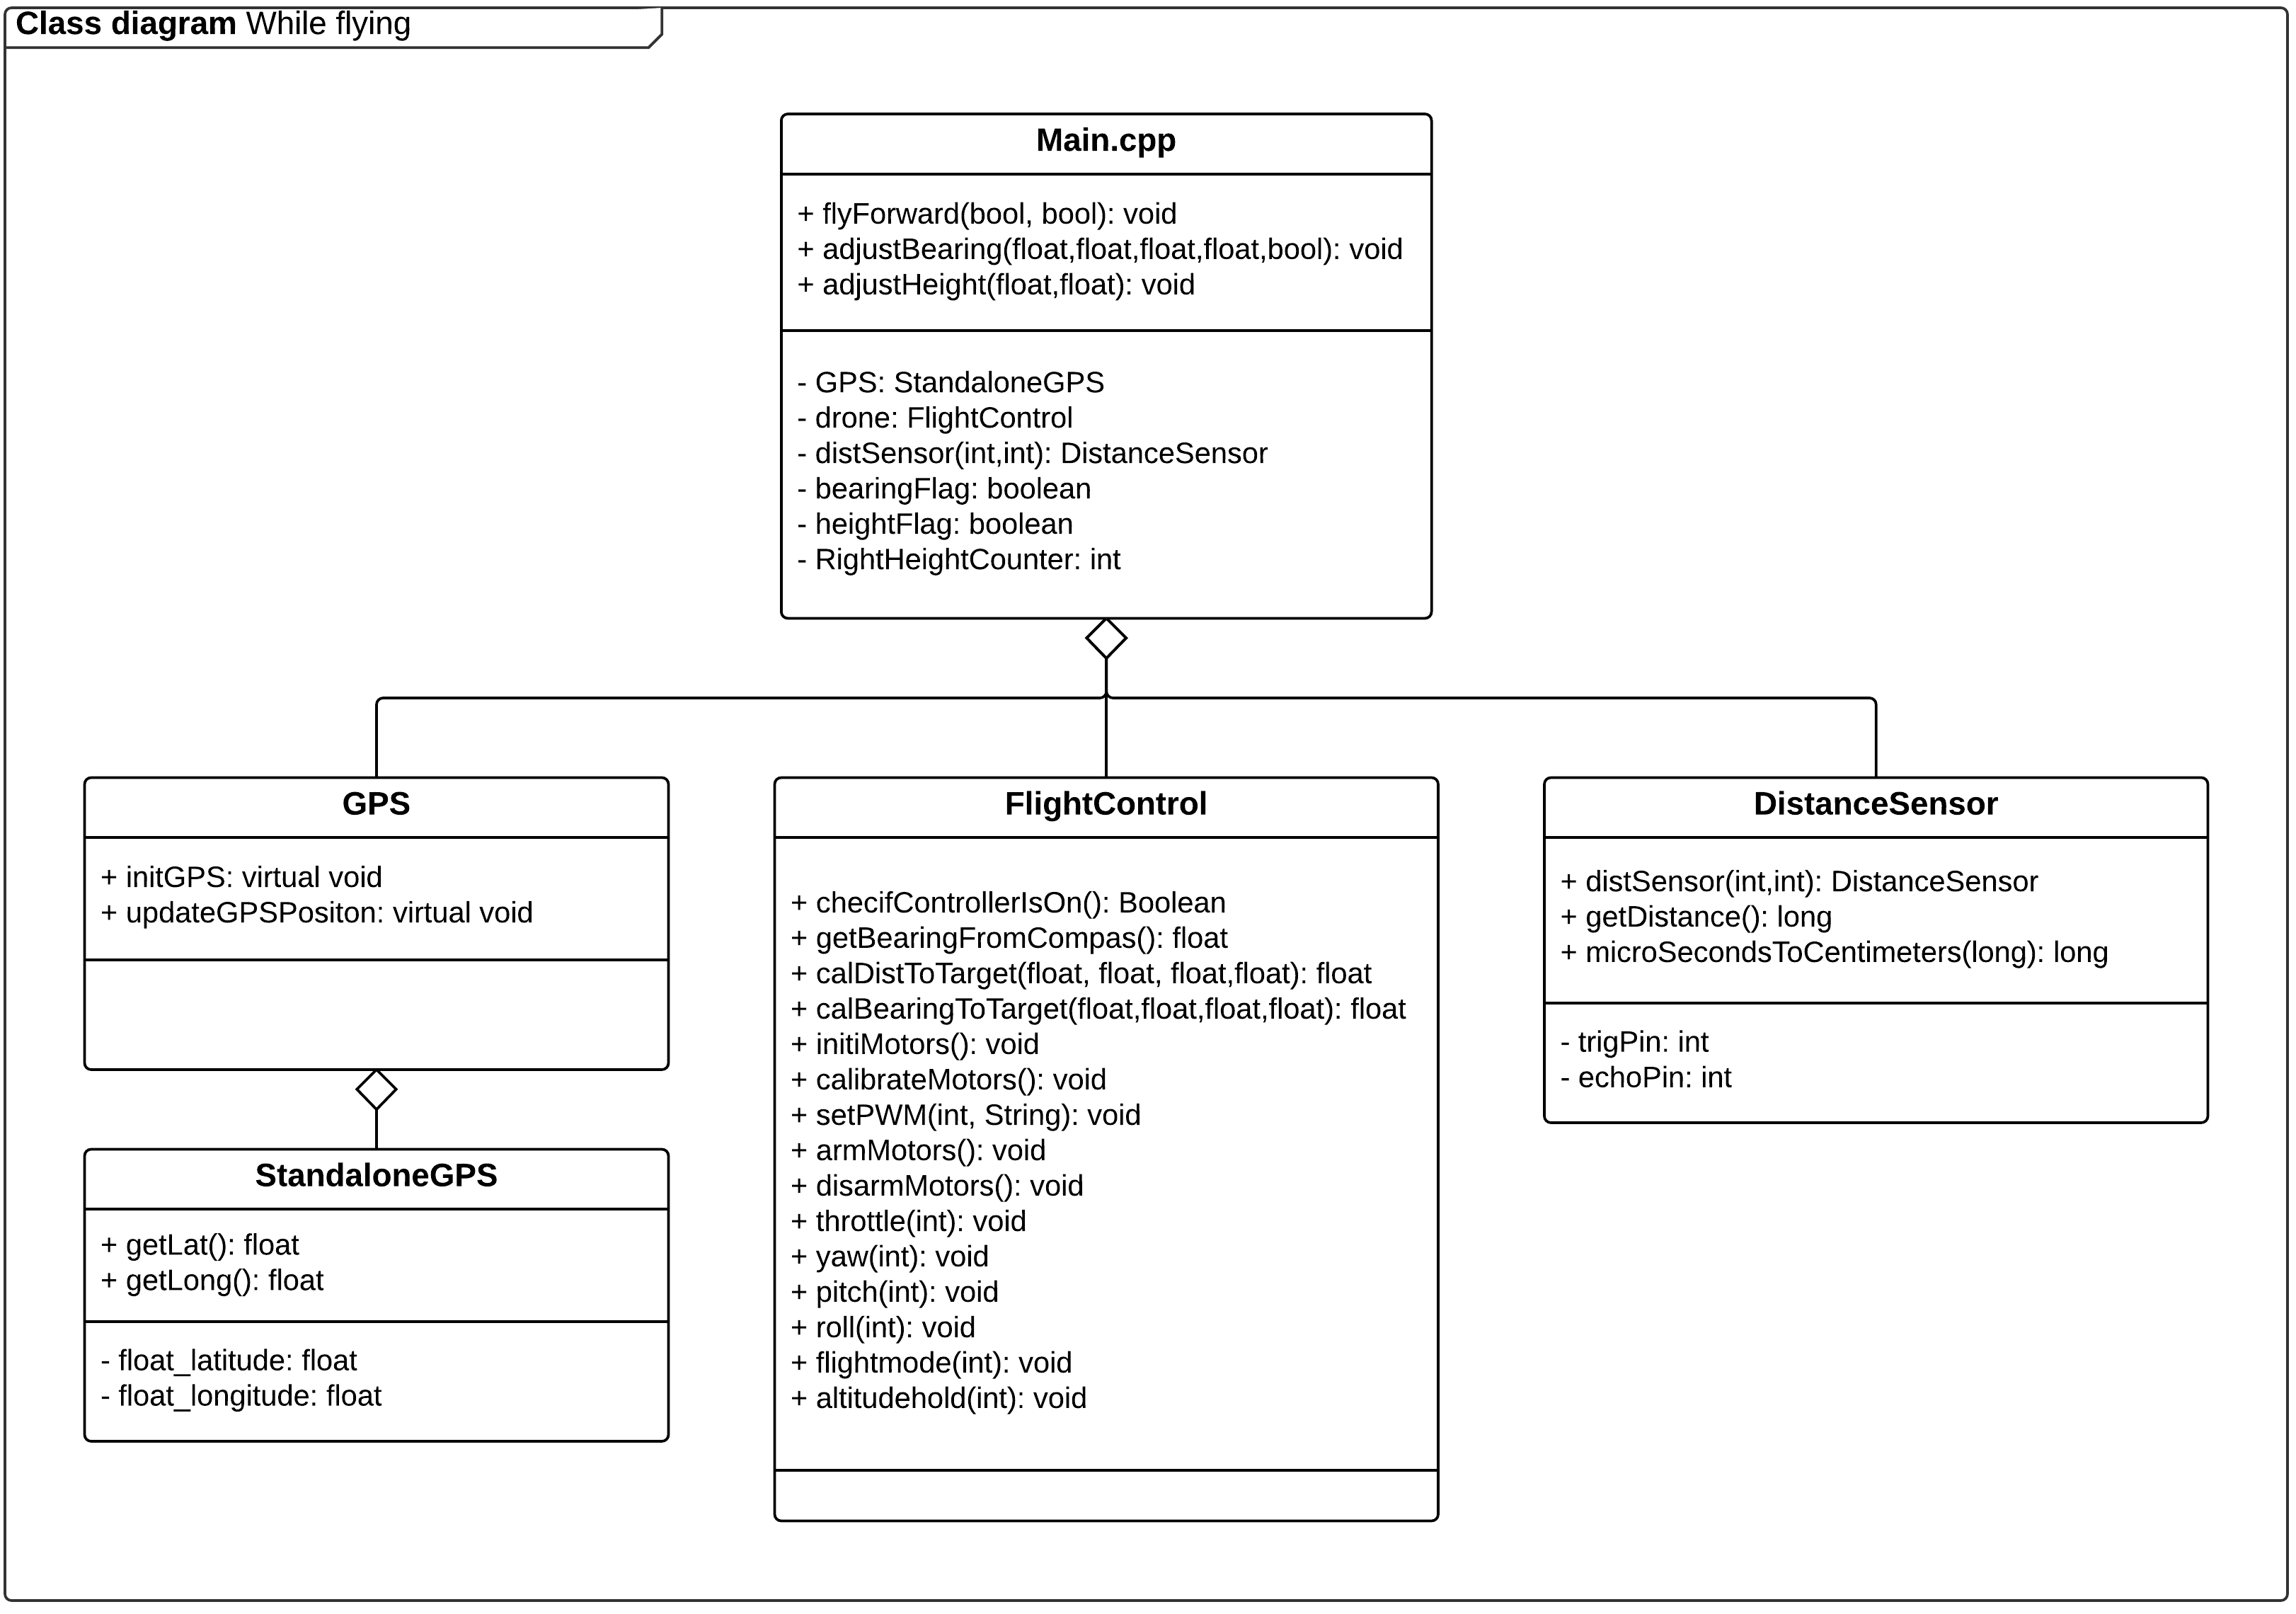
\includegraphics[width=1\textwidth]{Billeder/klasse_diagrammer/classdiagram_iteration2_fly.png}
	\vspace{0cm}
	\caption{Klassediagram drone}
	\label{fig:classDiagram_drone_underflyvning}
\end{figure}

\textbf{FlightControl} \\
Det er Flight Control klassen der har alt med styring af dronen at gøre, lige fra calibrering af motorerne til at hente data fra kompasset. 

\textbf{DistanceSensor} \\
DistanceSensor klassen bruges til at kontrollere de sensorer der er monteret på dronen. Her er det både sensorer til højdemåling og anti kollision. 

\textbf{GPS} \\
GPS klassen er implementeret som en abstract klasse, idet den ikke selv har nogle metoder den skal bruge, men med virtuelle metoder der sikrer at de implementeres i de afledte klasser. 
Init og updateGPSPosition er valgt til at være virtuelle klasser, hvilket gør at de skal implementeres uanset hvilken GPS der bruges. Klassen er lavet fordi der i udgangspunkt var mulighed for at bruge 3 forskellige slags GPS modes med 3G/GPS shieldet. 

\newpage
På Figur \ref{fig:classDiagram_3Gmodul} er der vist en udvidet klasse diagram for 3G modulet. På diagrammet vises de metoder og attributter der indgår i klasserne. 

\begin{figure}[H]
	\centering
	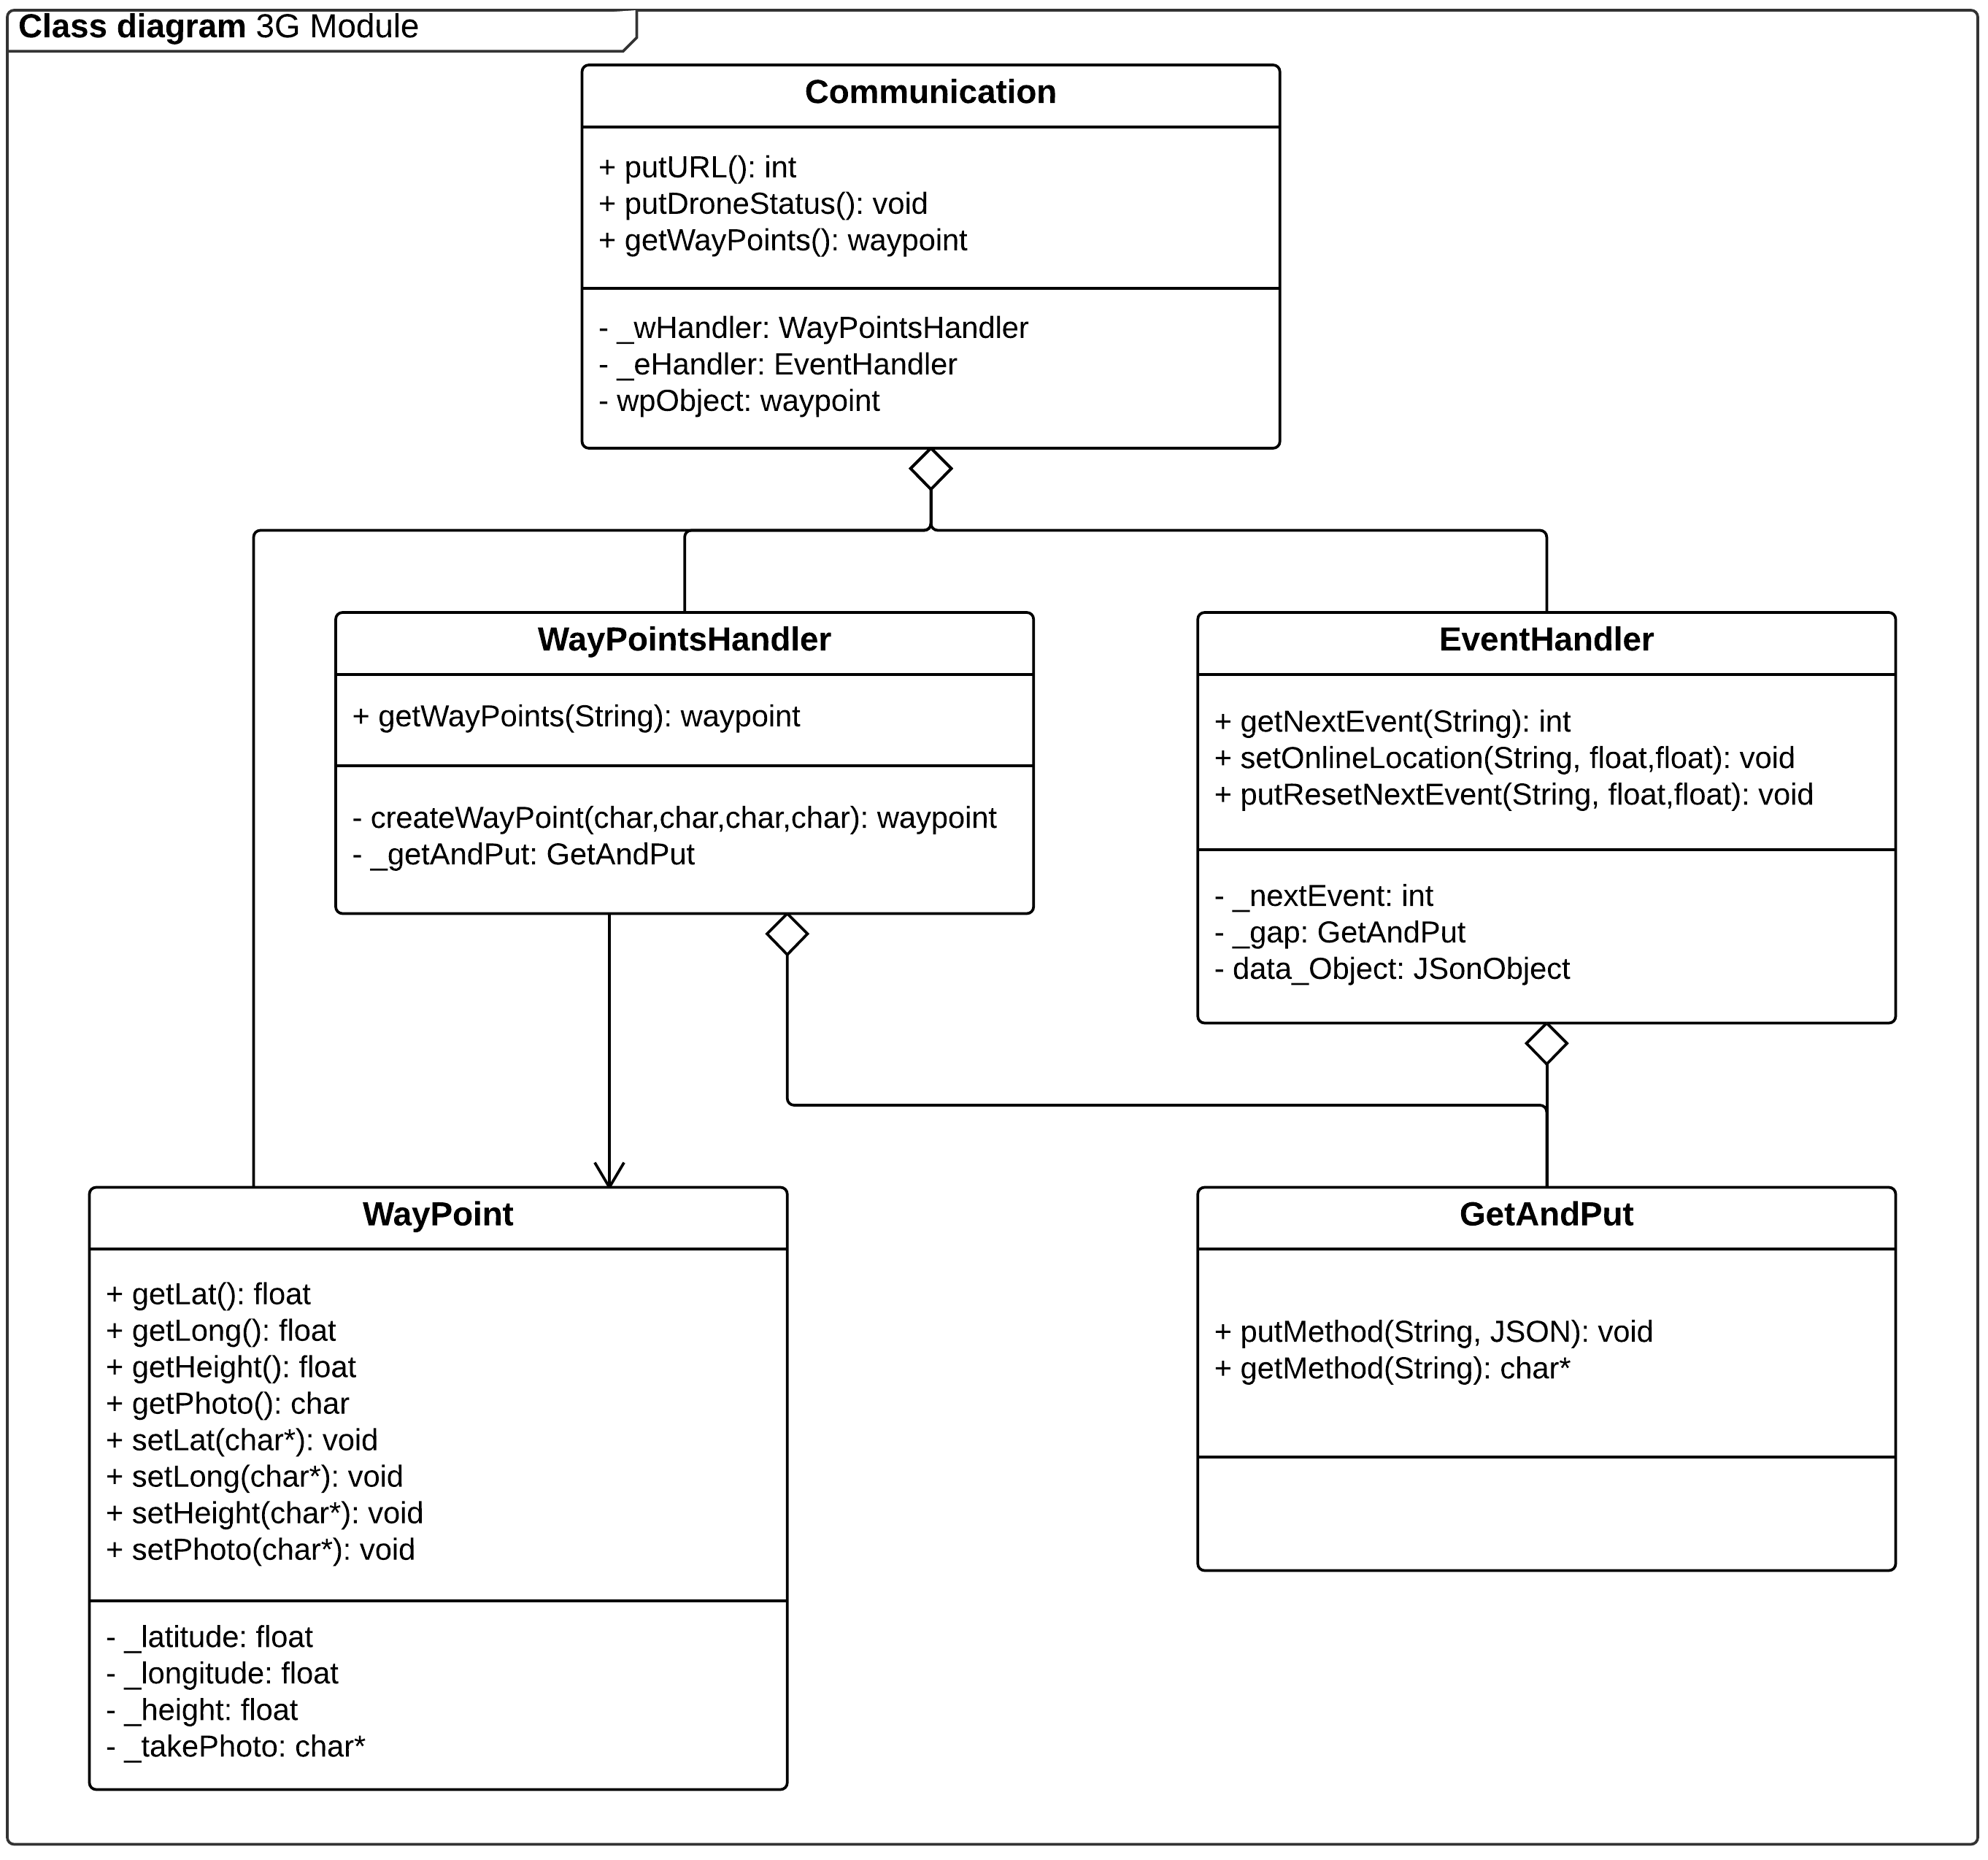
\includegraphics[width=1\textwidth]{Billeder/klasse_diagrammer/classdiagram_3gmodule.png}
	\vspace{0cm}
	\caption{Klassediagram 3G modul}
	\label{fig:classDiagram_3Gmodul}
\end{figure}


\textbf{GetAndPut} \\
GetAndPut klassen er den klasse der er tættest på hardwaren. Klassen indeholder de http metoder der bruges til kommunikation mellem dronen og serveren. 

\textbf{Communication} \\
Communication klassen er den øverste klasse og den håndterer sammen med andre klasser, alt der har med 3G at gøre.

\textbf{EventHandler} \\
EventHandleren er den klasse der håndterer Events. EventHandleren er bindeledet mellem communication- og GetAndPut klassen. EventHandleren sorterer eventID'et fra de data den modtager og returnerer værdien til communication klassen.

\newpage

\textbf{WayPointsHandler} \\
WayPointsHandler klassen er den klasse der håndterer de waypoints der hentes ned fra serveren. Klassen tager de waypoints den får fra serveren og gør dem tilgængeligt for resten af systemet. WayPointsHandleren bruger set metoderne i WayPoint klassen.

\textbf{WayPoint} \\
WayPoint klassen bruges til at kunne hente de forskellige waypoints ud af arrayet.  


\subsubsection*{Klassediagram webapplikation}
\vspace{-0.1cm}
På figur \ref{fig:classDiagram_home} ses klasse diagrammet tilhørende iteration to for websitet. Funktionaliteten er blevet udvidet med overblik over droner i systemet og deres status. Mulighed for at oprette events til den ønskede drone. 
\begin{figure}[H]
	\centering
	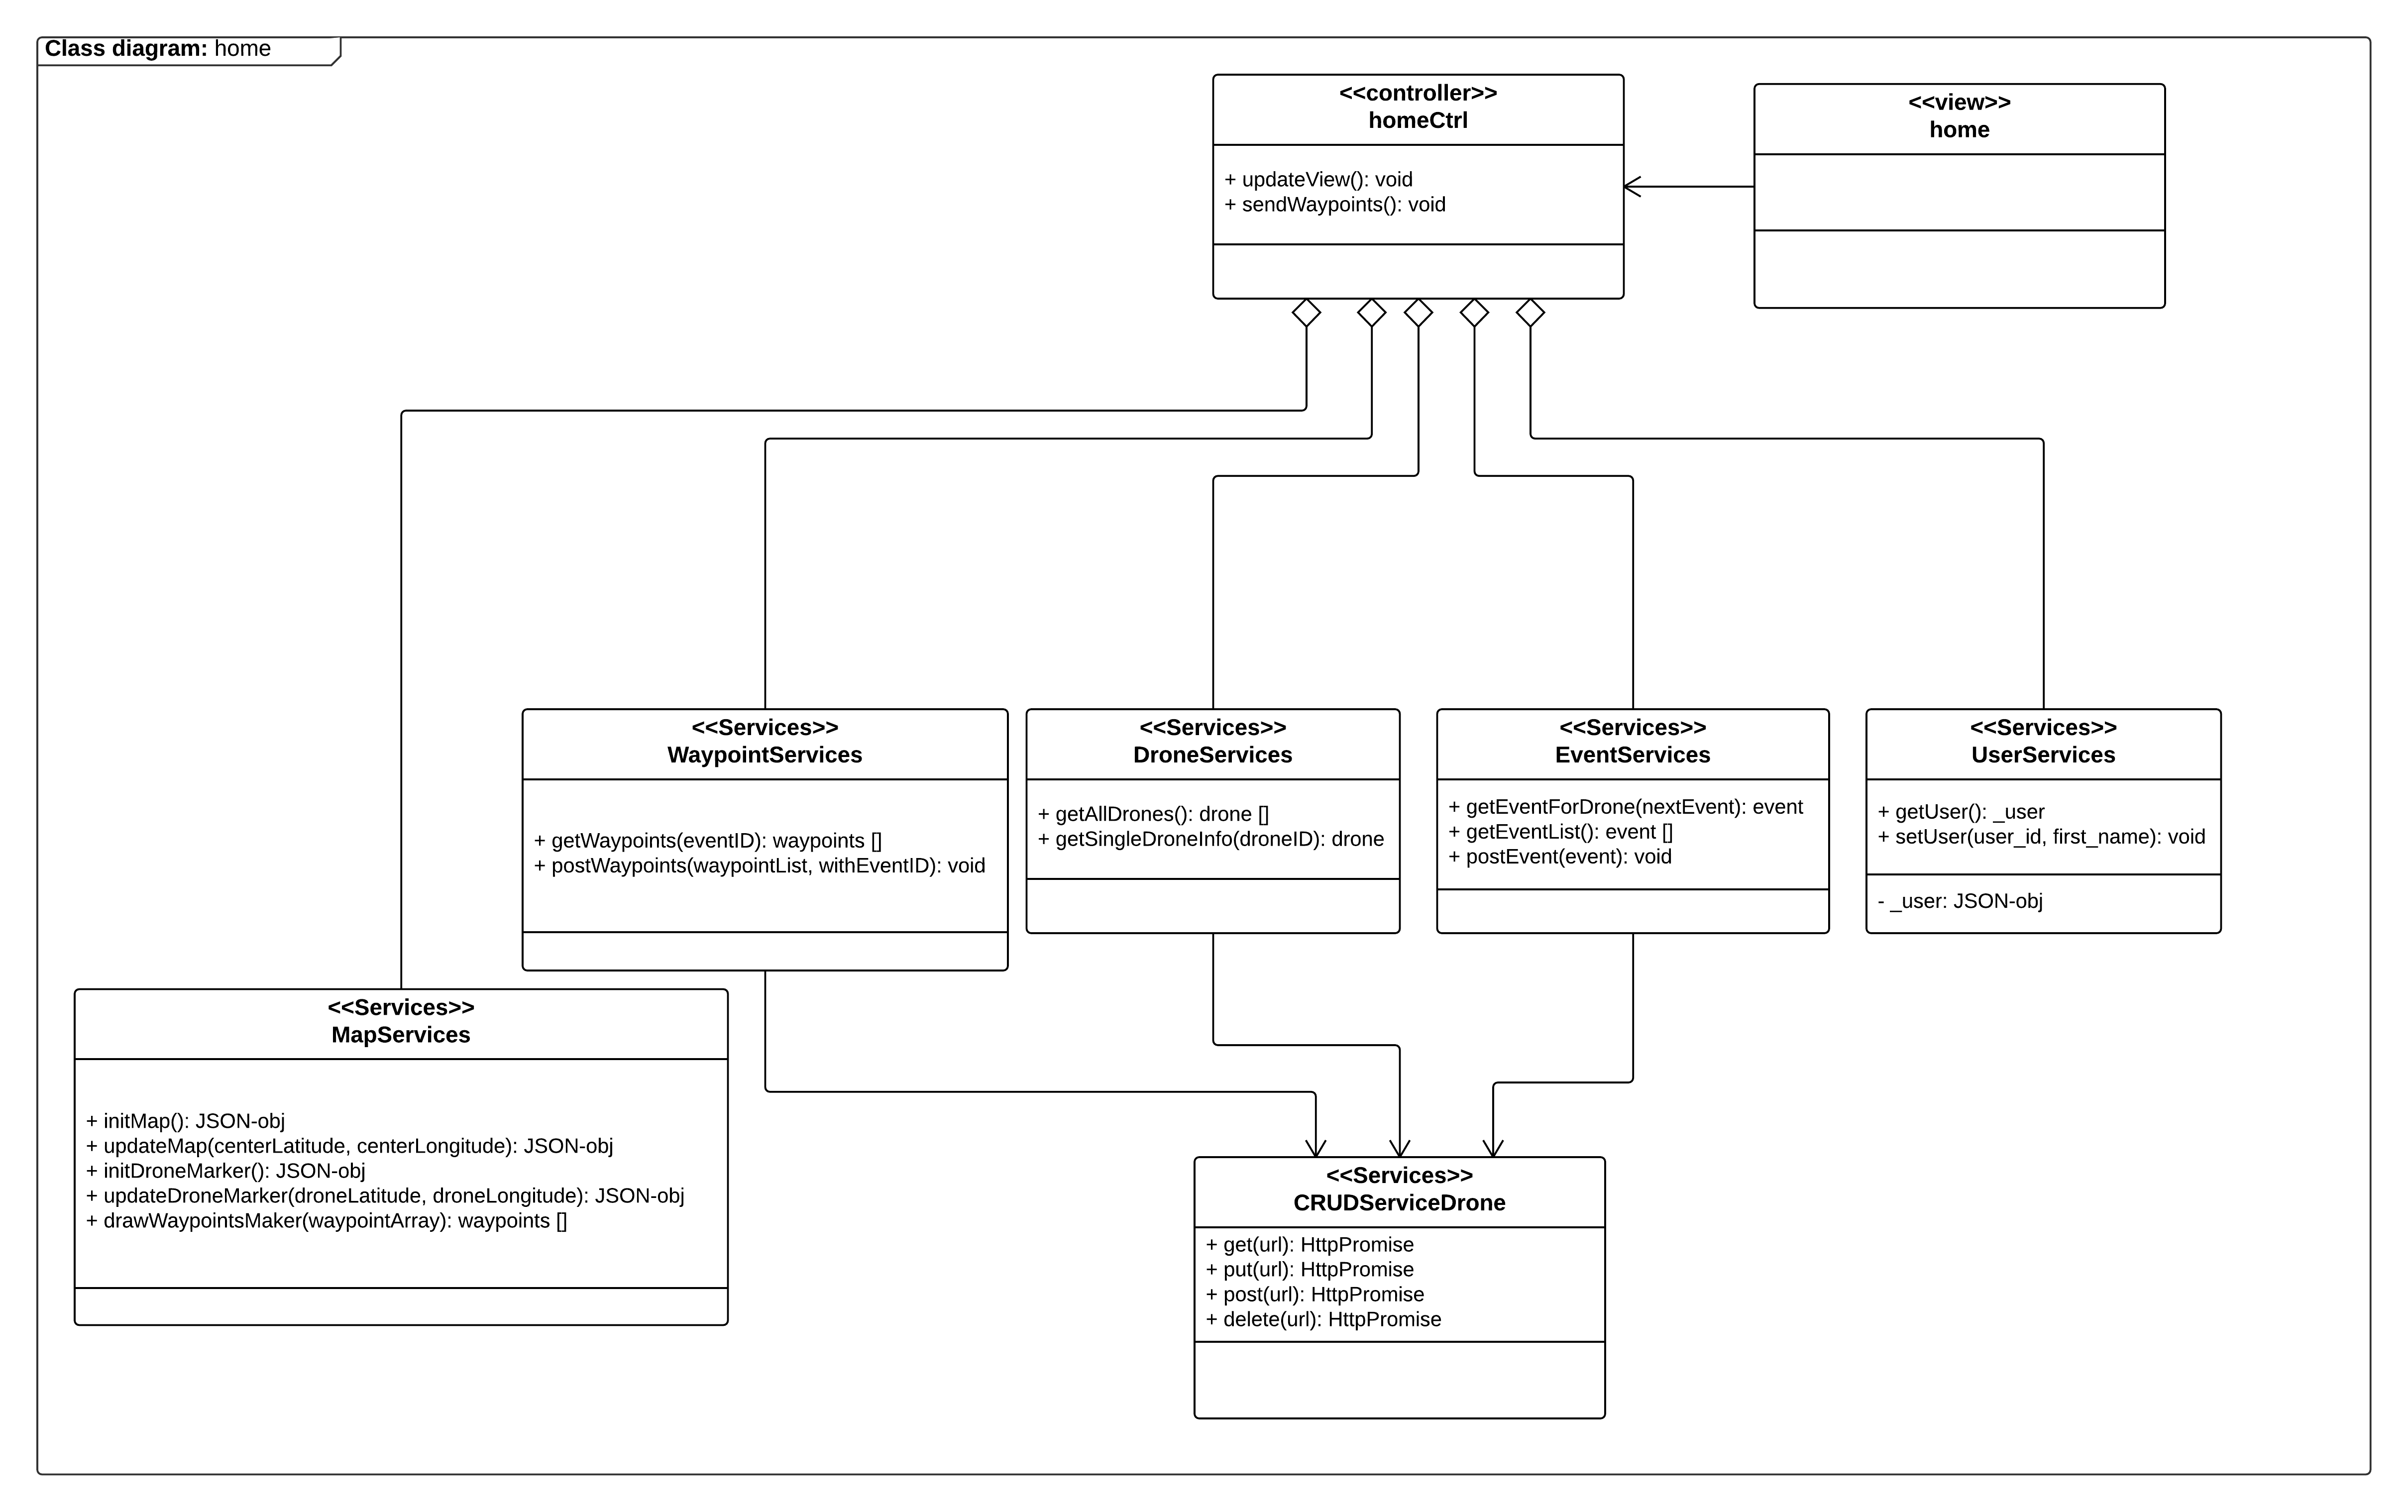
\includegraphics[width=1.\textwidth]{Billeder/klasse_diagrammer/home_class_diagram.png}
	\vspace{-0.5cm}
	\caption{Klassediagram home}
	\label{fig:classDiagram_home}
\end{figure}

\textbf{home}
Denne klasse er view'et tilhørende iteration to. Denne klasse sammen med homeCtrl skaber det endelig view som brugeren ser i sin browser når han besøger siden.

\textbf{homeCtrl}
HomeCtrl klassen er controller klassen til iteration to. Det er den eneste klasse der har direkte forbindelse til view'et, homeCtrl klassen deler også hukommelse med view'et igennem two-way-binding med scopes.

\textbf{DroneServices}
Denne klasse indeholder logikken om drone håndteringen. Den har ansvaret for at hente informationer omkring droner fra serveren via CRUDServiceDrone klassen.

\textbf{WaypointServices}
Denne klasse indeholder logikken om waypoint håndtering. Denne klasse henter henter waypoints tilhørende et event til controller klassen. Klassen bliver også brugt til at sende waypoints til serveren via CRUDServiceDrone klassen.

\textbf{EventServices}
Denne klasse indeholder logikken om event håndtering. Klassen bruges til at hente en event liste, et enkelt event for en givet drone og sende et nyoprettet event til serveren via CRUDServiceDrone klassen.

\textbf{MapServices}
Denne klasse indeholder logikken om map håndtering. Klassen bruges til at opdatere kortet i view'et, tegne waypoints og dronen på kortet.

\textbf{CRUDServicesDrone}
Denne klasse fungere som bindeled imellem server og webapplikation. Klassen indeholder alt logikken omkring kommunikation til serveren, alle der vil kommunikere med serveren i systemet skal benytte sig af denne klasse. Igennem denne service er det muligt at hente, opdater og poste data til serveren.

\textbf{UserServices}
Denne klasse blev oprettet i iteration et og bruges til at gemme information omkring hvilke bruger der er logget ind i systemet.